\documentclass[12pt]{article}
% Load packages
\usepackage{url}  % Formatting web addresses
\usepackage{ifthen}  % Conditional
\usepackage{multicol}   %Columns
\usepackage[utf8]{inputenc} %unicode support
\usepackage{amsmath}
\usepackage{amssymb}
\usepackage{epsfig}
\usepackage{epstopdf}
\usepackage{graphicx}
\usepackage[margin=0.1pt,font=footnotesize,labelfont=bf]{caption}
\usepackage{setspace}
%\usepackage{longtable}
\usepackage{colortbl}
%\usepackage{palatino,lettrine}
%\usepackage{times}
%\usepackage[applemac]{inputenc} %applemac support if unicode package fails
%\usepackage[latin1]{inputenc} %UNIX support if unicode package fails
\usepackage[wide]{sidecap}
%\usepackage[authoryear,round,comma,sort&compress]{natbib}
\usepackage[square,sort,comma,numbers]{natbib}
%\usepackage[authoryear,round]{natbib}
\usepackage{supertabular}
\usepackage{simplemargins}
\usepackage{comment}
\usepackage{lineno}
\usepackage{algorithm2e}

\urlstyle{rm}

%\textwidth = 6.50 in
%\textheight = 9.5 in
%\oddsidemargin =  0.0 in
%\evensidemargin = 0.0 in
%\topmargin = -0.50 in
%\headheight = 0.0 in
%\headsep = 0.25 in
%\parskip = 0.15in
%\linespread{1.75}
\doublespace

%\usepackage{geometry}
\usepackage{fullpage}

%\bibliographystyle{plain}
\bibliographystyle{msb}

\makeatletter
\renewcommand\subsection{\@startsection
	{subsection}{2}{0mm}
	{-0.05in}
	{-0.5\baselineskip}
	{\normalfont\normalsize\bfseries}}
\renewcommand\subsubsection{\@startsection
	{subsubsection}{2}{0mm}
	{-0.05in}
	{-0.5\baselineskip}
	{\normalfont\normalsize\itshape}}
\renewcommand\section{\@startsection
	{subsection}{2}{0mm}
	{-0.2in}
	{0.05\baselineskip}
	{\normalfont\large\bfseries}}
\renewcommand\paragraph{\@startsection
	{paragraph}{2}{0mm}
	{-0.05in}
	{-0.5\baselineskip}
	{\normalfont\normalsize\itshape}}
\makeatother

%Review style settings
%\newenvironment{bmcformat}{\begin{raggedright}\baselineskip20pt\sloppy\setboolean{publ}{false}}{\end{raggedright}\baselineskip20pt\sloppy}

%Publication style settings

% Single space'd bib -
\setlength\bibsep{0pt}

\renewcommand{\rmdefault}{phv}\renewcommand{\sfdefault}{phv}

% Change the number format in the ref list -
\renewcommand{\bibnumfmt}[1]{#1.}

% Change Figure to Fig.
\renewcommand{\figurename}{Fig.}

% Begin ...
\begin{document}
\begin{titlepage}
{\par\centering\textbf{\Large Model Identification of Leukemia Transcription Factor Networksr}}
\vspace{0.05in}
{\par \centering \large{ Katharine V. Rogers, Adithya Sagar, Holly A. Jensen,
and Jeffrey D. Varner$^{*}$}}
\vspace{0.10in}
{\par \centering \large{School of Chemical and Biomolecular Engineering}}
{\par \centering \large{Cornell University, Ithaca NY 14853}}
\vspace{0.1in}
{\par \centering \textbf{Running Title:}~}
\vspace{0.1in}
{\par \centering \textbf{To be submitted:}~\emph{}}
\vspace{0.5in}
{\par \centering $^{*}$Corresponding author current address:}
{\par \centering Jeffrey D. Varner,}
{\par \centering Professor, School of Chemical Engineering,}
{\par \centering 1158 Forney Hall, Purdue University, West Lafayette IN, 46907}
{\par \centering Email: jdvarner@purdue.edu}
{\par \centering Phone: (765) 496 - 0544}
\end{titlepage}
\date{}
\thispagestyle{empty}
\pagebreak
%%%%%%%%%%%%%%%%%%%%%%%%%%%%%%%%%%%%%%%%%%%%%%%%%%%%%%%%%%%%%%%%%%%%%%%%%%%%%%%%%%%%%%%%%%%%%%%%%%%%%%%%%%%
%%%%%%%%%%%%%%%%%%%%%%%%%%%%%%%%%%%%%%%%%%%%%%%%%%%%%%%%%%%%%%%%%%%%%%%%%%%%%%%%%%%%%%%%%%%%%%%%%%%%%%%%%%%
\section*{Abstract}


\vspace{0.5in}
{\noindent \textbf{Keywords:}~ leukemia, cancer, mathematical modeling}

\pagebreak

\setcounter{page}{1}

\linenumbers

\section*{Introduction}

It was suggested by Bailey, more than a decade ago, that qualitative and quantitative knowledge of complex biological systems could be achieved in the absence of complete structural and parameter knowledge \cite{Bailey2001}. Although this is true, the incomplete knowledge of biological phenomenon often limits the impact of computational models. Unknown or even disputed network structures can lead to incomplete fitting of computation models, requiring additional experiments and updating of the model. Since ODE kinetic models typically require extensive prior knowledge of network structure, rate constants and initial conditions \cite{Kholodenko2012}, often a single \textquotedblleft correct\textquotedblright $\:$  network structure is assumed. Villaverde  \textit{et al.} discussed three main strategies in the reverse engineering of dynamic models: (1) full network inference, (2) network selections, and (3) kinetic parameter estimations \cite{Villaverde:2014kl}. Strategy 1, where the kinetic model structure and kinetic parameters are unknown, is typically solved by identifying the model interaction network without dynamics and then identifying the kinetic parameters. In this study, we will consider strategy 2; we have an initial model network structure that will be perturbed to find modifications to fit the experimental data for six different leukemia cell lines. 

Leukemia is the 6th leading cause of cancer death in both males and females in the United States \cite{Siegel2015}. Approximately 72\% of cancer related leukemia deaths were caused by four main types of leukemia; acute lymphocyctic leukemia (ALL), chronic lymphocytic leukemia (CLL), acute myeloid leukemia (AML), and chronic myeloid leukemia (CML). ALL and CLL are characterized by accumulation of lymphocytes in the bone marrow, with ALL progressing at a faster rate (i.e. acute vs. chronic). ALL occurs in both children and adults and has a 90\% five year survival rate in children \cite{Hunger2015}, while CLL is rare in children and has a 66\% five year survival rate (2001-2009) \cite{Nabhan2014}.
The 10 year survival rate for CML has improved to 80-90\% due to the use of targeted treatments for BCR-ABL and adenosine triphosphate (ATP) \cite{Jabbour2014}.  
AML is characterized by the accumulation of abnormally differentiated cells of the hematopoietic system in the bone marrow and blood, with a survival rate of 35 to 40\% in adults under the age of 60 (5 to 15\% in patients older than 60) \cite{Dohner2015}.
AML is a group of extremely heterogeneous diseases, with over 200 known chromosome translocations and mutations in patient leukemic cells \cite{Gocek2012}.
The use of differentiation induction therapy agents like all-\textit{trans} retinoic acid (RA) and 1,25-dihyrodyvitamin D3 (D3) have been explored in many cancer cell types, including myeloid leukemias, and lung, liver, prostate, and breast cancer (RA treatment) \cite{Bushue2010,Tang2011} and in prostate, breast, colorectal, leukemia, and brain (D3 treatment) \cite{Cheung2012}.
Acute promyelocytic leukemia (APL), a subtype of AML, was once one of the most fatal forms of acute leukemia until the introduction of RA increased remission rates of patients to between 80 and 90 \% \cite{Coombs2015}.  
Failure of RA treatment can occur initially in patients with RA resistant variants (PLZF-RARA-positive APL), and relapse occurs in 5-20\% of cases due to the emergence of RA resistance.
To understand the response of multiple leukemia cell lines to RA and D3 treatments, we developed a network structure of well known transcription factors governing myelomonocytic lineage selection (granulocytic or monocytic). 

In this study we considered data from RA, D3, and RA plus D3 treatments on six human myeloid leukemia cell lines; (1) K562 (FAB M1), (2) HL60 (FAB M2), (3) NB4 (FAB M3), (4) U937 (FAB 5), (5) HL60 R38+ and (6) HL60 R38- (5 and 6 are described previously \cite{Jensen2013}). 
K562, a CML cell line with a Bcr-Abl fusion protein \cite{Lozzio1975}, was used as a control because the cells are not responsive to both RA \cite{Robertson1991} and D3 treatment \cite{Munker1986}. 
HL60 cells, an AML cell line, are lineage-bipotent myelobasts \cite{Fontana1981,Dalton1988} that can differentiate to either granulocytic lineage (using RA) or monocytic lineage (using D3). 
The two RA-resistant HL60 cell lines, R38+ and R38-, were described previously \cite{Jensen2013,Jensen2014}.
NB4, an APL cell line, are highly RA-responsive, but require combination treatments for monocytic differentiation (i.e. low response to D3) \cite{Bhatia1994,Testa1994}.
U937, histiocytic lymphoma cell line, are highly responsive to D3 induced monocytic differentiation, but have ambiguous differentiation effects due to RA (either monocytic or granulocytic) \cite{Olsson1982, Nakajima1996, Defacque1995}.
The model network contained two inputs (RA and D3) and 18 main species. 
We included two receptors, reinoic acid receptor alpha (RAR$\alpha$) and vitamin D receptor (VDR), but excluded their heterodimer receptor pair, retinoid receptor (RXR), for simplicity (assumption RXR is readily available). 
Also, included in the model were transcription factors important in myelomonocytic lineage selection (listed in Table \ref{Leukemia_TF_Network}). 
Finally upstream markers for differentiation were included, including CD38, CD11b, CD14, G1/GO cell cycle arrest and inducible oxidative metabolism. 
CD38 and CD11b are myelomonocytic markers and CD14 is a monocytic specific marker. 

In this study we first determined that a network structure of a small three node protein model could be identified with sufficient experimental data. 
A model structure search in combination with particle swarm optimization to determine parameter values narrowed down total possible model structures from 19683 to twenty. 
After additional experimental data was implemented, we were able to find the synthetic model structure with no \textit{a priori} knowledge. 
Next we investigated possible network structures for transcription factor and upstream markers in six leukemia cell lines treated with RA and D3 (data from \cite{Jensen2015}). 
The upstream markers CD38 and CD11b (myelomonocytic markers) and CD14 (monocytic specific marker) were included in the model.  
Also, included in the model were transcription factors important in myelomonocytic lineage selection.
Starting from an initial best model structure curated from literature sources, we were able to improve the model fits for six leukemia cell lines versus experimental data.  

\section*{Results}

\subsection{Three Node Example Network}

To determine if we could distinguish between possible model structures, we began by first modeling a simple three protein node network. The model we designated as the true model is shown in Figure \ref{fg:3node_models}A and the results for the synthetic data generated are given in Figure \ref{fg:TrueModelData}. 
All proteins in the model could act as either transcription factors or transcription repressors. 
The two examples of transcriptional regulation, activation and repression, are given in Figure \ref{fg:3node_models}D. 
Assuming no prior knowledge, other than number of nodes and inducer location, we were able to narrow down possible network structures with just one experiment and ultimately determine the true network structure with a small set of additional experiments (Table \ref{exp_table}). 
For an n node protein network with three possible interactions between nodes (activation, inhibition, or no interaction) and allowing for self regulation (i.e. $P_{1}$ can be a transcription factor for itself), we had a total of $3^{n^{2}}$ possible structures, where n is the number of protein nodes. 
The simple n = 3 case had a total of 19683 possible model structures, which we exhaustively searched and determined a best fit parameter set for each model using particle swarm optimization. 
For particle swarm optimization we designated a ten particle system and 30 operations, for 300 total iterations. 
The initial ten particles were each a set of parameters containing 35 randomized parameters (20 control parameters and 15 kinetic parameters). 
Using the data from five species (one saved for validation) in experiment 1 (Table \ref{exp_table}), we narrowed our results to the 20 best model structures (top 0.1\%).   
For these 20 best models, we ran a second particle swarm optimization with 300 total iterations to determine if a better solution could be found.
In this case we started with ten particles randomized from the best parameter set from each model obtained from the first trial.  
As shown in Figure \ref{fg:Top20Models}, the true model was not selected as the best fit and we did not find the  \textquotedblleft true\textquotedblright $\:$ parameter set. 
The top model was similar to the true model with two additional interactions and two opposite sign interactions (i.e. activation instead of inhibition) (Fig. \ref{fg:3node_models}B).
Therefore, by using data from just one experiment we were able to obtain a subset of 20 possible model structures. 

From the possible 20 model structures we wanted to determine if we could narrow down the possibilities to one structure with the use of additional experimental data. 
All top 20 models show qualitatively the correct response (Fig. \ref{fg:Top20Models}) and therefore, the simulation error could be caused either by a model structure issue or a parameter set estimation issue (did we find the correct parameters?). 
The top 20 models have many features in common (Fig. \ref{fg:3node_models_Table}): (1) All 20 models designated $P_{1}$ as a transcription factor activator for species two, (2) 19 models showed $P_{2}$ inhibits itself, (3) 20 models showed $P_{2}$ as a transcriptional regulator (activator or repressor) for species three, with four having the opposite interaction (i.e. repression instead of activation), and (4) 18 models showed $P_{3}$ regulated itself, but 12 of these cases are opposite (activation instead of repression).
Many of the structures also had added interactions: (1) ten models added regulation from $P_{3}$ to species two, (2) eight models added self-regulation of $P_{1}$ (all activation), and (3) eight models added regulation of species three by $P_{1}$.
After studying the possible structures we performed two additional experiments to obtain synthetic data (Table \ref{exp_table}). 
In experiment two an inducer was added at t=100 A.U. and the binding domain of $P_{2}$ was inhibited (i.e. $P_{2}$ could not act as a transcription factor). 
Finally, in experiment three an inducer was added every 24 A.U. starting at t = 100 A.U., to represent step inputs on the system. 
Again we ran a particle swarm optimization method to find a new best fit parameter set for the top 20 models, this time using a total of three experiments and five species per experiment to calculate experimental error (Table \ref{3_node_objective}).
With the additional two experiments we were able to exclude the previous top model (Fig. \ref{fg:3node_models}B).
In figure \ref{fg:Top20Models_Exp2}C and \ref{fg:Top20Models_Exp2}F, we see that the previous top model (in blue) does not qualitatively fit mRNA or protein data for species three. 
The true model (red) is the second best fitting model after optimization with three experiments, while the new top fitting model is in green.   
In experiment two, $mRNA_{3}$ decreased due to the inhibition of $P_{2}$ activity ($P_{2}$ is a transcription factor activator for $mRNA_{3}$ in the true model). 
The previous top model (3147) was not able to obtain this result due to the incorrect interaction between $P_{2}$ and species three (inhibition instead of activation). 
The new top model (Fig. \ref{fg:3node_models}C) had one additional interaction that occured between $P_{3}$ and species two. 
After finding that the control parameter value, $\kappa_{3,2}$, was 9.9e-7 (essentially zero), for this interaction we were able to ignore the additional interaction (in equation \ref{transferfunction}, if $\kappa_{3,2}$ = 0 then $f_{3,2}$ = 0). 
Therefore, with using only three experiments and 15 objective functions we were able to obtain the correct model structure after exhaustively searching all 19683 possible structures.
From the small three node network we determined that the correct model structure could be identified with sufficient experimental data after an exhaustive network search.

\subsection{Leukemia Transcription Factor Network}

Next we investigated possible network structures for transcription factor and upstream markers in six leukemia cell lines treated with RA and D3 (data from \cite{Jensen2015}).
The six cell lines, K562, HL60, NB4, U937, HL60 R38+ and HL60 R38-, had diverse reactions to the stimuli and thus, we assumed that network structures could differ between cell lines.
The leukemia transcription factor network with two inducers (RA and D3), contained 42 differential equations (RXR was included but set to zero in this case), 652 control parameters, and 90 kinetic parameters. 
In this case, with n = 18 protein nodes, if no prior knowledge was assumed, other than number of nodes and inducer location, we would have a total of $3^{18^{2}}$ possible model structures. 
To narrow down our search space we first assumed proteins which do not act as transcription factors always have no interaction from the protein to another species: CD38, CD11b, CD14 and p47. 
Also, we designated the protein Gfi-1 as always acting as a repressor if the interaction existed.
Next we created an initial guess transcription factor network by searching the literature, which is shown in Figure \ref{fg:Initial_TF_Network} (interactions and references shown in Table \ref{Leukemia_TF_Network}).
We began by calculating a top parameter set for each cell line using this initial network structure. 
A top parameter set was calculated using particle swarm optimization with 35 particles and 90 iterations per particle, for a total of 3150 iterations. 
Simulation data for each cell line was compared to 39 objective functions found in Table \ref{Leukemia_TF_objective}.
After finding the parameter set with the lowest error for each model based on this initial structure, we then perturbed the model by randomly changing one to three edges in the model from our initial best guess to either no interaction (0), negative interaction (-1), or positive interaction (1).
Again we used particle swarm optimization to find a new best parameter set for the updated model.
If the error was less then the previous model we accepted the new model, and in the next iteration we would perturb this new model structure. 
Through this method, we looked at approximately 300 model structures for each cell line and were able to improve model fits compared to the initial model structure.   



Through model and parameter optimization we discovered improved network structures for the six cell lines: K562, HL60, NB4, U937, HL60 R38+ and HL60 R38-. 
The new network structures showed improved fits against a subset of the experimental data. 
For example the new model structure of the HL60 R38- cell line was able to accurately predict the increase in VDR concentration due to a D3 stimulus and RA+D3 stimulus which was missed in the original structure (Figure \ref{fg:R38-HL60_Experiment}).
The new model structure for the HL60 cell line was able to predict the CD38 expression shift due to RA and RA + D3 stimulus, but still missed the D3 stimulus experiment (Figure \ref{fg:WTHL60_Experiment}).
In the NB4 case of CD11b concentration we again missed the D3 stimulus experiment, but were able to improve the results of the RA and RA + D3 stimulus experiments (Figure \ref{fg:NB4_Experiment}).
Change in PU.1 concentration due to RA, D3, and RA + D3 treatments was accurately modeled with the new K562 model structure (Figure \ref{fg:K562_Experiment}). 
Training experiments involving AhR in U937 cells and C/EBP$\alpha$ in HL60 R38+ cells are also shown (Figure \ref{fg:U937_Experiment} and \ref{fg:R38+HL60_Experiment}).
To improve the model fits many perturbations (adding, deleting, or switching edges) were made to the initial network structure for each cell line.
For the K562 cell line, unresponsive to RA and D3, 100 changes were made to our initial best network structure (Table \ref{K562_Model}). 
The model structure for the NB4 cell line, which is highly responsive to RA, contained 90 changes (Table \ref{NB4_Model}).
For HL60 cells, 91 edges were changed in the model structure (Table \ref{WTHL60_Model}).
The two RA resistant HL60, R38- and R38+, models had 76 and 74 changes, respectively (Table \ref{HL60-R38_Model} and Table \ref{HL60+R38_Model}).
Finally, the U937 model had 41 network changes in the best model solution (Table \ref{U937_Model}).
Taken together, through a combination of network perturbations we were able to better predict a subset of experiments in six leukemia cell lines: K562, HL60, NB4, U937, HL60 R38+ and HL60 R38-. 
We also developed new model structures specific to each cell line from our initial shared model structure guess.


\section*{Discussion}

In this study, we developed a method for determining protein node network structures from experimental data with incomplete biological knowledge. 
The models described transcriptional regulation due to the input of inducers. 
First we were able to determine a toy three node protein network structure by searching through all possible structures and using particle swarm optimization to optimize parameters. 
The network structure was narrowed down to a subset of 20 models using data from one experiment and eventually found using two additional experiments. 
In total, 15 objective experiments were used for training and three experiments were saved for prediction. 
Of the top 20 network structures found many of the edges were conserved including: (1) All 20 models designated $P_{1}$ as a transcription factor activator for species two, (2) 19 models showed $P_{2}$ inhibits itself, (3) 20 models showed $P_{2}$ as a transcriptional regulator (activator or repressor) for species three, with four having the opposite interaction (i.e. repression instead of activation), and (4) 18 models showed $P_{3}$ regulated itself, but 12 of these cases are opposite (activation instead of repression). In many cases additional interactions were added. 
By adding data from two additional experiments to the training, we were able to narrow down the results further with the true model as the second best result. 
After determining the two models differed in only one additional interaction, which was essentially zero due to the kinetic parameter, we were able to exclude this interaction and therefore found the true model.
One note, we were not able to find the true parameter set that was used to obtain the synthetic data with the number of iterations performed.
Additional parameter estimation and the use of an ensemble of parameter sets may be necessary to find a more optimal parameter solution. 
From this we determined that the correct network structure of a small transcriptional regulation network could be found with enough experimental data and model iterations.

Next we applied this method to determine transcription factor network structures for six leukemia cell lines: K562, HL60, NB4, U937, HL60 R38+ and HL60 R38-.  
All six cell lines have different reactions to RA, D3, and RA + D3 stimuli. 
RA, a current treatment for APL, is limited by RA resistance, variable efficacy in different cell types, and lack of understanding of the mechanism of action. 
Jensen \textit{et al.}, studied transcriptional regulation in six leukemia cell lines to determine the changes in critical transcription factors in myelomoncytic differentiation between cell lines \cite{Jensen2015}. 
By using the experimental data from this study we wanted to find new network structures in each cell line and therefore, better understand the critical changes in the development of new cancer subtypes.  
The initial network structure curated from literature contained transcription factors as well as upstream markers for myelomonocytic lineage selection.
Network perturbations included the addition and deletion of interactions as well as switching an interaction (i.e. upregulates to represses). 
We found new top network structures for all six cell lines and network perturbations can be found in Tables \ref{K562_Model} - \ref{U937_Model}.
Interestingly, there was no edge change that was consistent between all cell lines.
Three network changes were made to five of six cell lines: switched or deleted AhR upregulates PU.1 (edge 100), added C/EBP$\alpha$ upregulates VDR (edge 110), and switched or deleted C/EBP$\alpha$ upregulates PU.1 (edge 118). 
Looking through the network perturbations we were able to find some literature evidence for a few interactions.
For example upregulation of AP-1 by Oct1 was added to the network structure of four cell lines (K562, NB4, and WTHL60) and has been studied in \cite{Ullman1993}. 
This interaction was also added to the HL60 R38- model, except in this case AP-1 was repressed by Oct1. 
By continuing to look through the data we can determine more biologically relevant interactions found in the new models. 
The new leukemia cell line specific transcription factor models were able to improve the fit of experimental data from a subset of experiments. 
Some issues that need to be resolved include the fitting of many D3 only experiments. 

The initial leukemia transcription factor network was assembled after extensive literature review and hand curation of the biochemical interactions. 
One note was that interactions came from additional cell lines, including breast and prostate cancer, and therefore these interaction may or may not exist in leukemia cell lines.
In this study we tried to determine new network structures by perturbing a best guess initial model network from literature.
Data was limited to thirteen different proteins, out of 18 included in the model.
Additional experiments with mRNA data would be useful in determining final model structures as we modeled mRNA.
A population study should be performed on the flow cytometry data to see if population dynamics can be fit, not just single cell response.
To improve the model network search a machine learning method could be used in which after each model perturbation error is calculated and based on this error a probability is given to the edges perturbed.
For example, if we perturb edge ten and error triples, we can give the probability of making this step in the future very low. 
Also, it would be interesting to look at edges that have very little effect on model error. 
Another element that should be added to the model is the determination of granulocytic or monocytic differentiation in the cell lines in response to RA and D3 treatments. 
The ratio of PU.1 to C/EBPA$\alpha$ determines granulocytic vs. monocytic lineage selection \cite{Dahl2003}.
CD38 and CD11b are myelomonocytic markers and CD14 is a monocytic specific marker.
Overall the goal was to determine network structures to explain varying responses to RA and D3 treatment in six leukemia cell lines.
The network structures found can be studied further to determine important functional changes between cell lines.


\section*{Materials and Methods}

\subsection{Formulation of Network Model Equations}

For each motif of N protein nodes, a mRNA and protein balance for each node is written as:
\begin{equation}\label{}
\frac{dm_{j}}{dt}=r_{X,j}v_{X,j} - k_{d,j}m_{j} - \mu m_{j} + \lambda
\end{equation}
\begin{equation}\label{}
\frac{dp_{j}}{dt}=r_{T,j}v_{T,j} - k^{'}_{d,j}p_{j} - \mu p_{j} \qquad
\end{equation}
where j = 1,2,3 ... N. Degradation rates are given as $k_{d,j}$ and $k^{'}_{d,j}$, and $\lambda$ denotes a basal mRNA production rate.\\
The balances governing cellular infrastructure such as RNA polymerase (RNAP) and ribosomes (RIBO) are given by: 
\begin{equation}\label{}
\frac{dRNAP}{dt}=(\alpha - RNAP)\mu
\end{equation}
\begin{equation}\label{}
\frac{dRIBO}{dt}=(\beta - RIBO)\mu
\end{equation}
where $\alpha$ and $\beta$ are constants.
Balances governing a given inducer $I_{\pi}$ and cellular growth rate $\mu$:
\begin{equation}\label{}
\frac{dI_{z}}{dt}=\delta
\end{equation}
\begin{equation}\label{}
\frac{d\mu}{dt}=0
\end{equation}
There are a total of 2N + $\Pi$ + 3 differential equations for each motif, where $\Pi$ is the number of inducers in the network. 

The terms $r_{X,j}$ and $r_{T,j}$ denote the rate of transcription and translation respectively and are given by:
\begin{equation}\label{}
r_{X,j} = k_{X,j}(RNAP)\mu_{j} \quad
\end{equation}
\begin{equation}\label{}
r_{T,j} = k_{T,j}(RIBO)m_{j}\omega_{j}
\end{equation}

where $\mu_{j}$ and $\omega_{j}$ describe the allocation of RNAP and RIBO resources to the expression and translation of node j:
\begin{equation}\label{}
\mu_{j} = k_{X,j}(RNAP)\left[\sum_{i}k_{X,i}(RNAP)\right]^{-1} 
\end{equation}
\begin{equation}\label{}
\omega_{j} = k_{T,j}(RIBO)m_{j}\left[\sum_{i}k_{T,i}(RIBO)m_{i}\right]^{-1}
\end{equation}
The rate of expression and translation for node j is modified by control variables which describe the regulatory inputs controlling the node. One assumption is that translation is not actively regulated, thus $v_{T,j}$ = 1. Transcription may be regulated by other proteins in the motif. If the expression of species j had m activating factors and n repressive factors, the control term was modeled as a mean:
\begin{equation}\label{}
v_{j} = \frac{\left(\sum\limits_{i\in{j^{+}}}u_{i,j} + \sum\limits_{i\in{j^{-1}}}d_{i,j}\right)}{(m+n)}
\end{equation}
where:
\begin{equation}\label{}
u_{ij} = f_{ij} 
\end{equation}
\begin{equation}\label{}
d_{ij} = 1 - f_{ij}
\end{equation}
The quantities $\j^{+}$ and $j^{-}$ denote the sets of activating and repressive factors for gene j.
There are many possible functional forms for $0 \leq f_{ij}(\mathcal{Z}) \leq 1$. 
Each individual transfer function took the form:
\begin{equation}\label{transferfunction}
f_{i}(x) = \frac{\kappa_{ij}^{\eta}\mathcal{Z}_{j}^{\eta}}{1+\kappa_{ij}^{\eta}\mathcal{Z}_{j}^{\eta}}
\end{equation}
where $\mathcal{Z}_{j}$ denotes the abundance of the j factor (e.g. protein abundance), and $\kappa_{i,j}$ and $\eta$ are control parameters. The $\kappa_{i,j}$ parameter was a gain parameter and $\eta$ was a cooperatively parameter (similar to a HIll coefficient). 

The small three protein network with one inducer contained 10 differential equations, 20 control parameters, and 15 kinetic parameters. 
For the small three protein network the model equations were encoded using the Python programming language and solved using the ODEINT routine of the SciPy module \cite{Jones2001}. 
The leukemia transcription factor network with two inducers (RA and D3), contained 42 differential equations (RXR was included but set to zero in this case), 652 control parameters, and 90 kinetic parameters. 
Due to the increased size of the network, the model equations in this case were encoded using the Julia programming language \cite{BEKS14} and solved using the CVODE solver in the SUNDIALS library \cite{Hindmarsh2005}.

\subsection{Estimation of top parameter sets using Particle Swarm Optimization (PSO)}

We used particle swarm optimization to estimate top parameter sets for each model. 
Particle swarm optimization employs a population of particles with their own coordinates, velocity and best fit error to find a global best fit error \cite{Eberhart1995}.  

The mean squared error, $\eta$, of parameter set $\mathbf{k}$ for training objective $j$ was defined as:    

\begin{equation}
\eta_j(\mathbf{p}_k) = \frac{1}{N}\sum_{i}^{N}\frac{(\hat{x}_{i,j} - \beta_j x(\mathbf{p_k})_{i,j})^2}{\hat{\sigma}^2_{i,j}}
\end{equation}

The symbol $\hat{x}_{i,j}$ denotes scaled experimental observations (from training objective j) while $x(\mathbf{p_k})_{i,j}$ denotes the simulation output (from training objective j). The quantity $i$ denotes the sampled time-index or condition, and $N$ denotes the number of time points or conditions for experiment j. The standard deviation, $\hat{\sigma}_{i,j}$, was calculated from at least three experimental repeats. $\beta_j$ is a scaling factor which is required when considering experimental data that is accurate only to a multiplicative constant. In this study, the experimental data used for training and validation was typically band intensity from immunoblots, where intensity was estimated using the ImageJ software package \cite{Abramoff2004}. The scaling factor used was chosen to minimize the normalized squared error \cite{Brown2003}:

\begin{equation}
\beta_j = \frac{\sum_{i}(\hat{x}_{i,j}x_{i,j}/\hat{\sigma}_{i,j}^2)}{\sum_{i}(x_{i,j}/\hat{\sigma}_{i,j})^2}
\end{equation} 

By using the scaling factor, the concentration units on simulation results were arbitrary, which was consistent with the arbitrary units on the experimental training data. All simulation data was scaled by the corresponding $\beta_j$. 

The cost function for the optimization problem can be expressed as: 

\begin{equation}
\text{minimize  }K(\mathbf{p}_k) = \sum_{i}^{L}\eta_j(\mathbf{p}_k)
\end{equation} 

where L is the number of objective functions used for training. 

To begin PSO we randomly initialized a swarm of $\mathcal{K}$-dimensional particles (represented as $\mathbf{x}_{i}$), which correspond to a $\mathcal{K}$-dimensional parameter vector.
After running the necessary simulations, for each initial particle we calculated the particle error for all L objective functions, the total particle error (K), and the velocity vector (initially set to zero).  
Next we determined the global best error (i.e. the lowest K value for all particles) and global best particle position. 
For each operation after initialization, the velocity ($\mathbf{v}_{i,j}$) and position ($\mathbf{x}_{i,j}$) of each particle were updated by the following equations:

\begin{equation}
\mathbf{v}_{i,j} = \theta \mathbf{v}_{i,j-1} + \mathcal{A} \mathbf{r}_{1} (\mathcal{L}_{i} - \mathbf{x}_{i,j-1}) + \mathcal{B} \mathbf{r}_{2}(\mathcal{GL} - \mathbf{x}_{i,j-1})
\end{equation} 
\begin{equation}
\mathbf{x}_{i,j} = \mathbf{x}_{i,j-1} + \mathbf{v}_{i,j} 
\end{equation} 
where ($\theta$, $\mathcal{A}$, $\mathcal{B}$) are adjustable parameters, $\mathcal{L}_{i}$ denotes best local solution found by particle $i$ up until function evaluation $j-1$, and $\mathcal{GL}$ denotes the best global solution up until function evaluation $j-1$.
The quantities $\mathbf{r}_{1}$ and $\mathbf{r}_{2}$ denotes uniform random vectors with the same dimension as the number of unknown model parameters ($\mathcal{K}x1$). 

\clearpage

Again for each new particle position we calculated the particle error for all L objective functions, the total particle error (K), and the velocity vector. 
Using a greedy search we updated $\mathcal{L}_{i}$ and $\mathcal{GL}$ by the following rules: 
\begin{algorithm}
\If{$K_{i,j} < K_{best,i}$}{  	
  \BlankLine
  $K_{best,i} = K_{i,j}$\\
  $\mathcal{L}_{i} = \mathbf{x}_{i,j}$ 
  \BlankLine
  \If{$K_{i,j} < K_{globalbest}$}{
   \BlankLine
   $K_{globalbest} = K_{i,j}$\\
   $\mathcal{GL} = \mathbf{x}_{i,j}$
   \BlankLine
  }
}
\end{algorithm}

After J total operations we saved $\mathcal{GL}$ and $K_{globalbest}$ for the given model network structure. 

\clearpage

\bibliography{References_TFModel}

\clearpage

\begin{figure}\centering
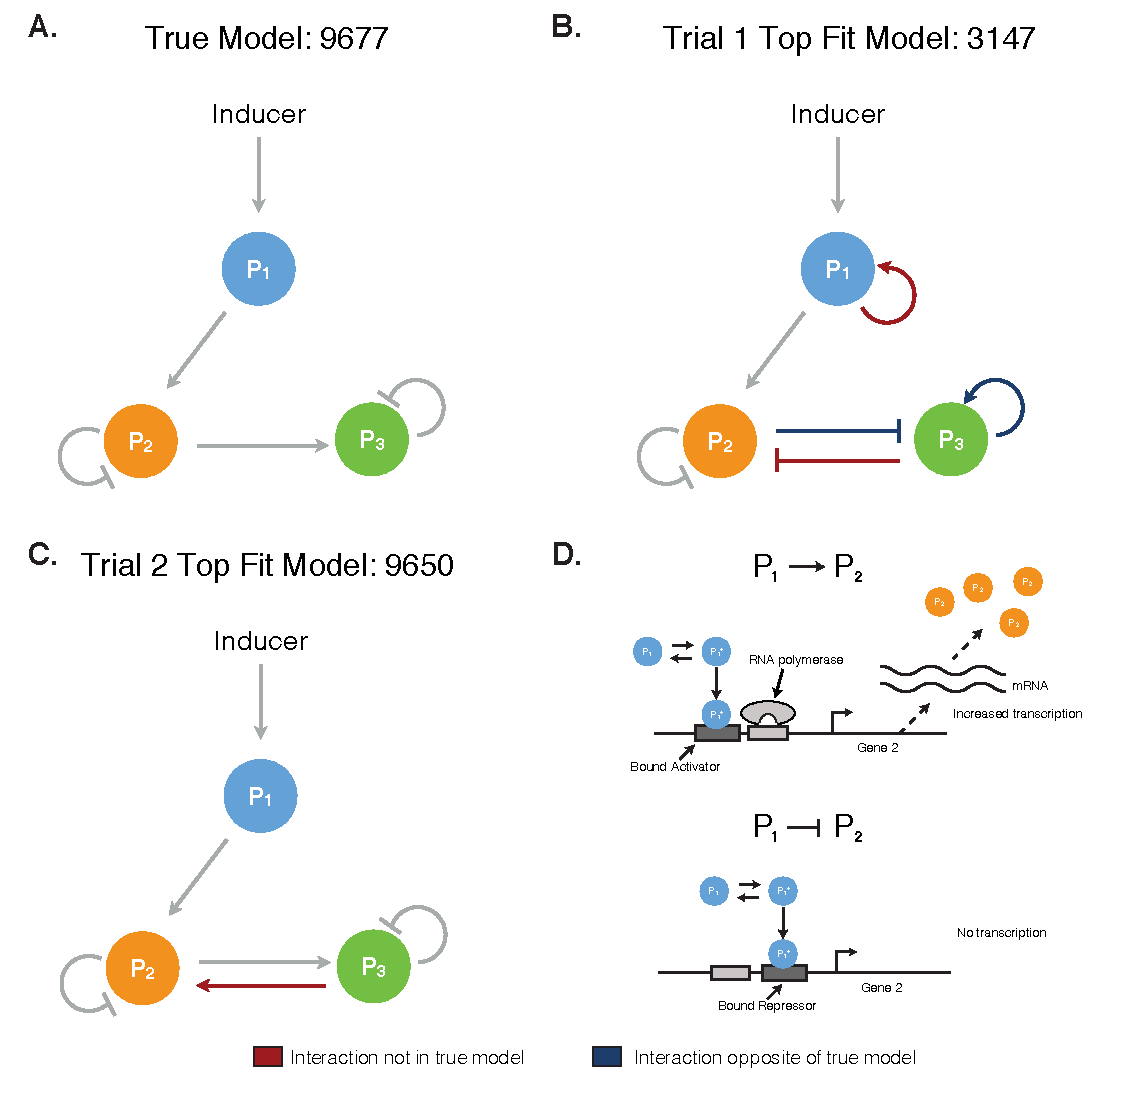
\includegraphics[width=1.0\textwidth]{./figs_chp3/Fig1_3node_models.pdf}
\caption{Model for three node protein network. Arrows denote activation and lines denote inhibition. The model includes three proteins ($P_{1}$, $P_{2}$, and $P_{3}$), the corresponding mRNA ($mRNA_{1}$, $mRNA_{2}$, and $mRNA_{3}$), RNA polymerase (RNAP), ribosomes (RIBO), and Inducer. $\bf{A.}$ The true model for the three node protein network. $\bf{B.}$ The best fit model after parameter estimation using data from only one experiment. $\bf{C.}$ The best fit model after parameter estimation using data from experiments 1, 2 and 3. Red lines denote interactions not in original model and blue lines denote interactions that are opposite of the original model. $\bf{D.}$ Gene transcription activation and repression in the model (figure modified from \cite{Alon2007}).}
\label{fg:3node_models}
\end{figure}

\clearpage

\begin{figure}\centering
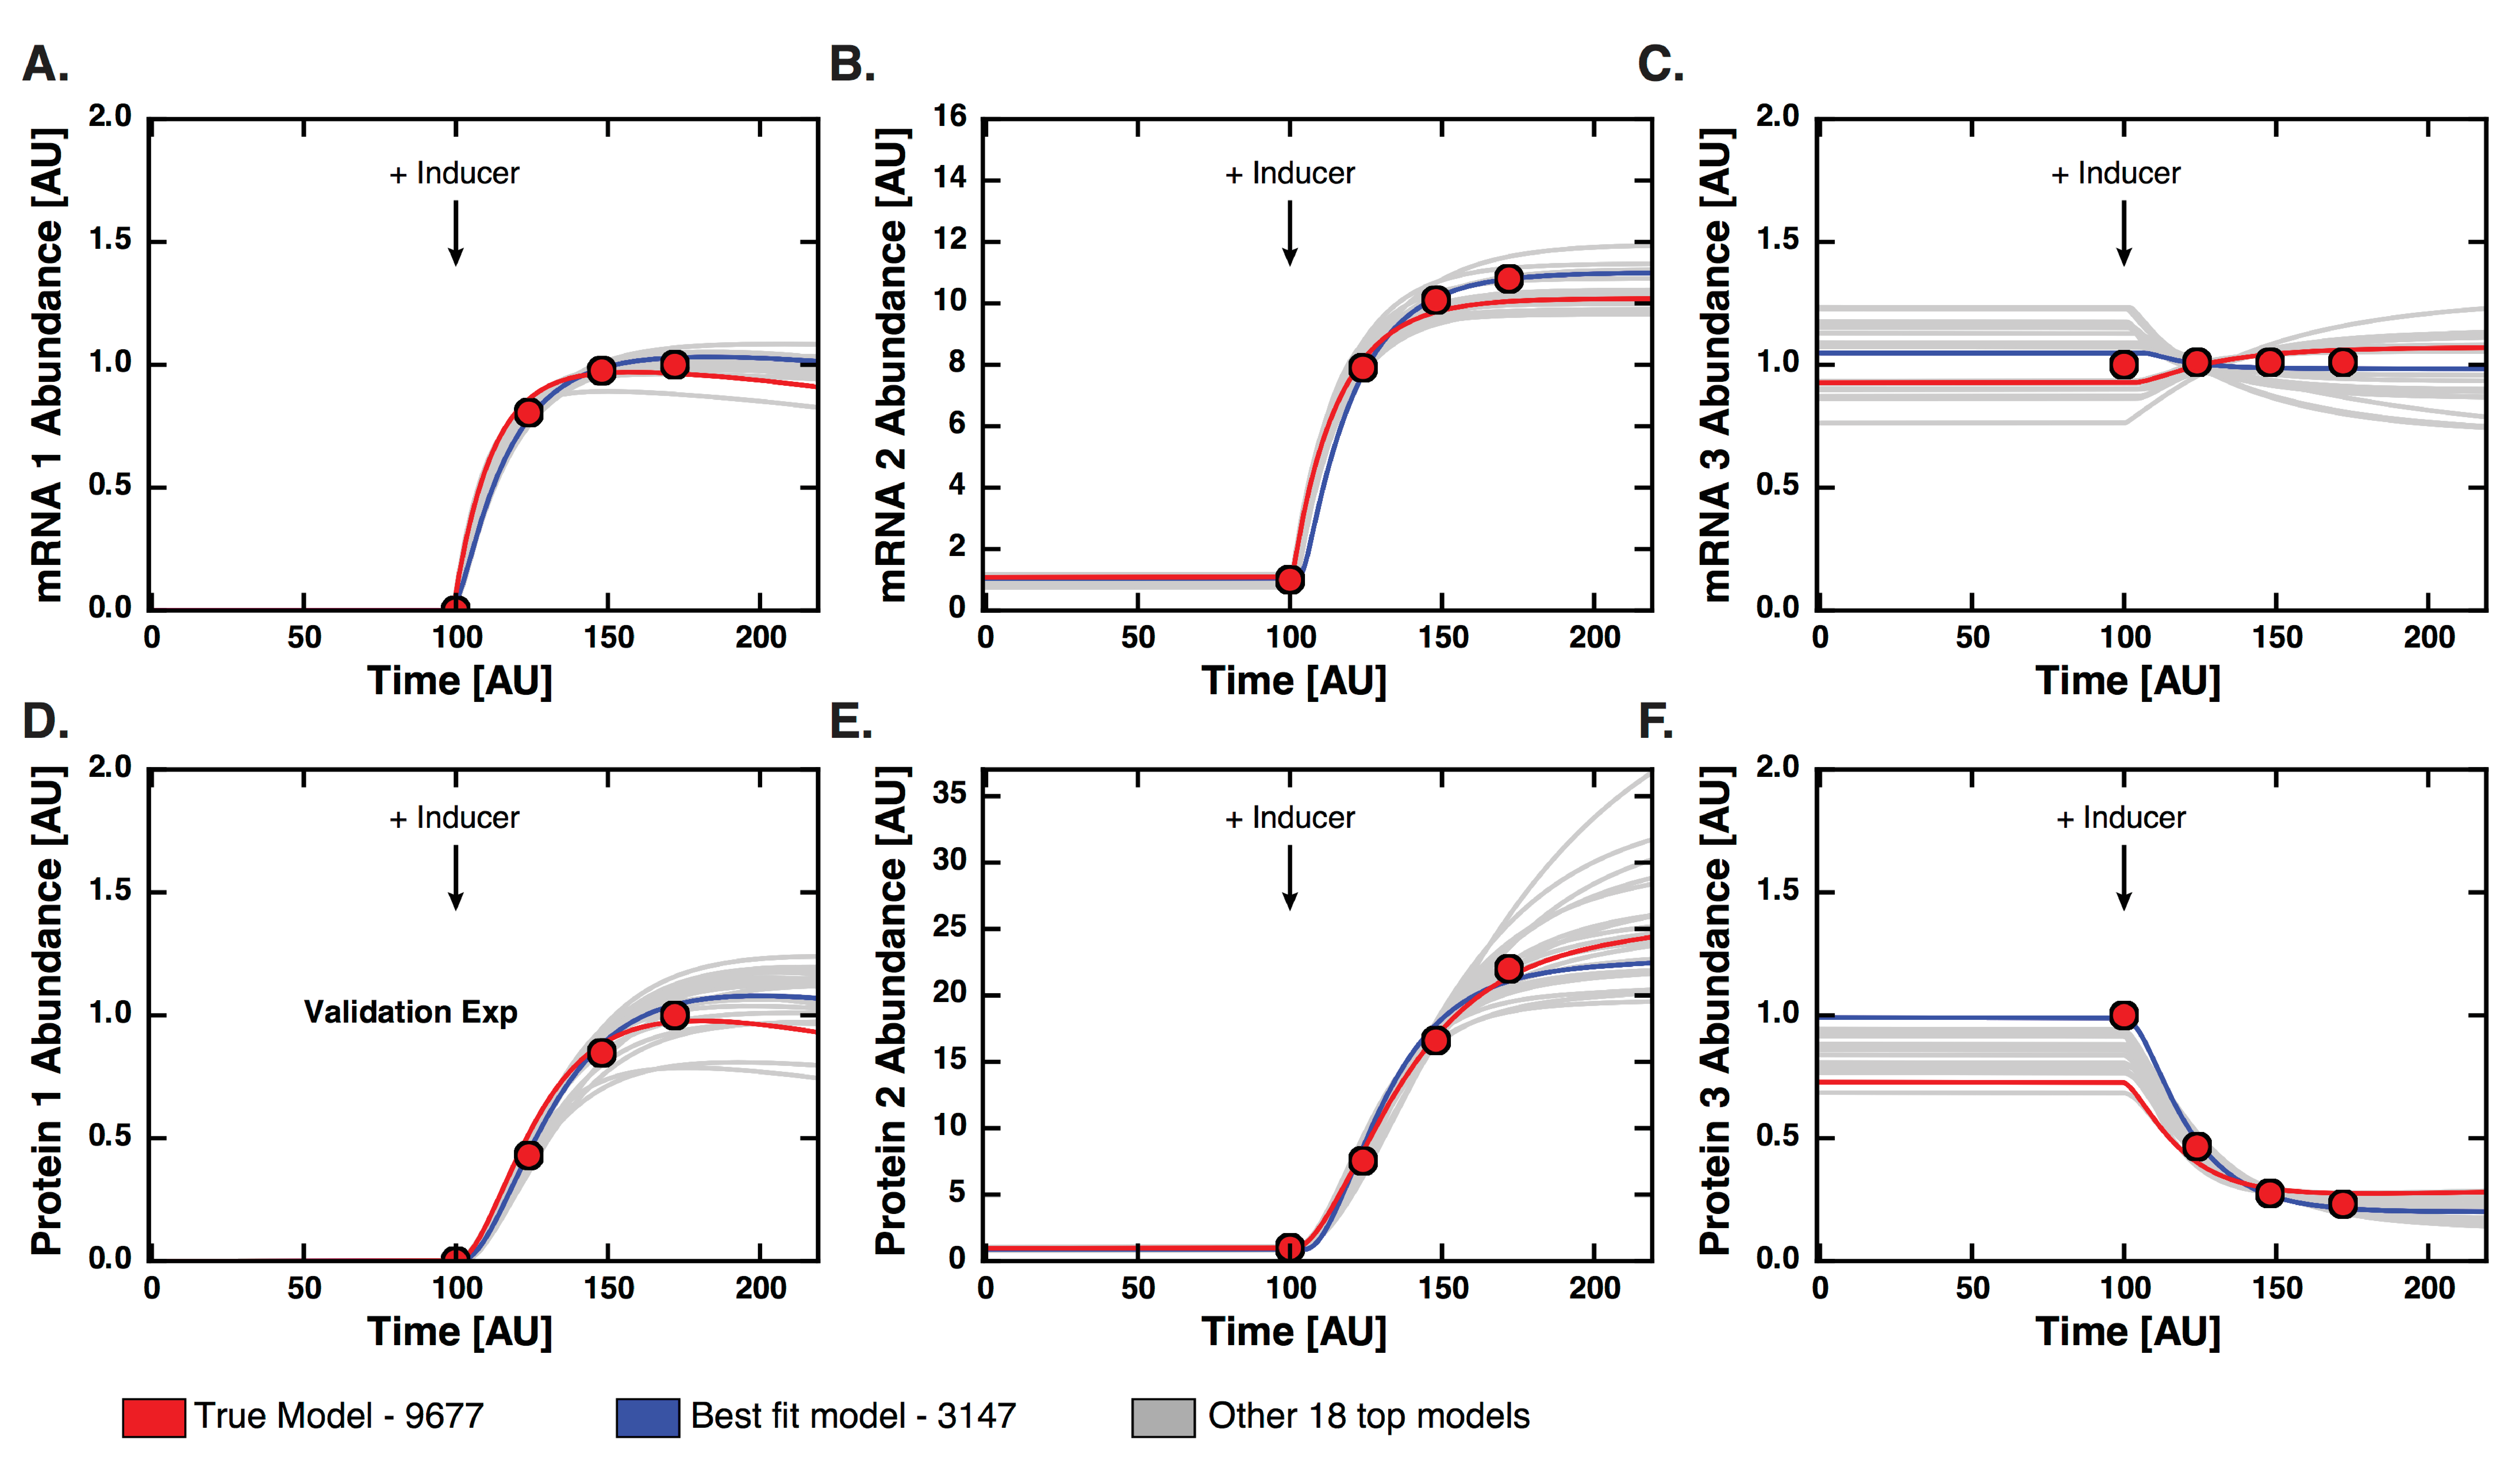
\includegraphics[width=1.0\textwidth]{./figs_chp3/Fig2_Top20_Models_2.pdf}
\caption{Experiment 1 results for the top 20 models with respective best parameter sets determined from particle swarm optimization. In experiment 1, inducer was added at Time = 100. $\bf{A, B, C.}$ Plots of mRNA concentration profiles for species 1, 2, and 3 after inducer added at Time = 100. $\bf{D.}$ Plot of protein concentration profile for species 1 which was used for validation. $\bf{E, F.}$ Plots of protein concentration profiles for species 2 and 3. Red dots denote synthetic experimental data used for fitting. Red lines represent the true model with optimized parameters, blue denotes the best fitting model (\ref{fg:3node_models}B), and the grey lines represent remaining top 18 models.}
\label{fg:Top20Models}
\end{figure}

\clearpage

\begin{figure}\centering
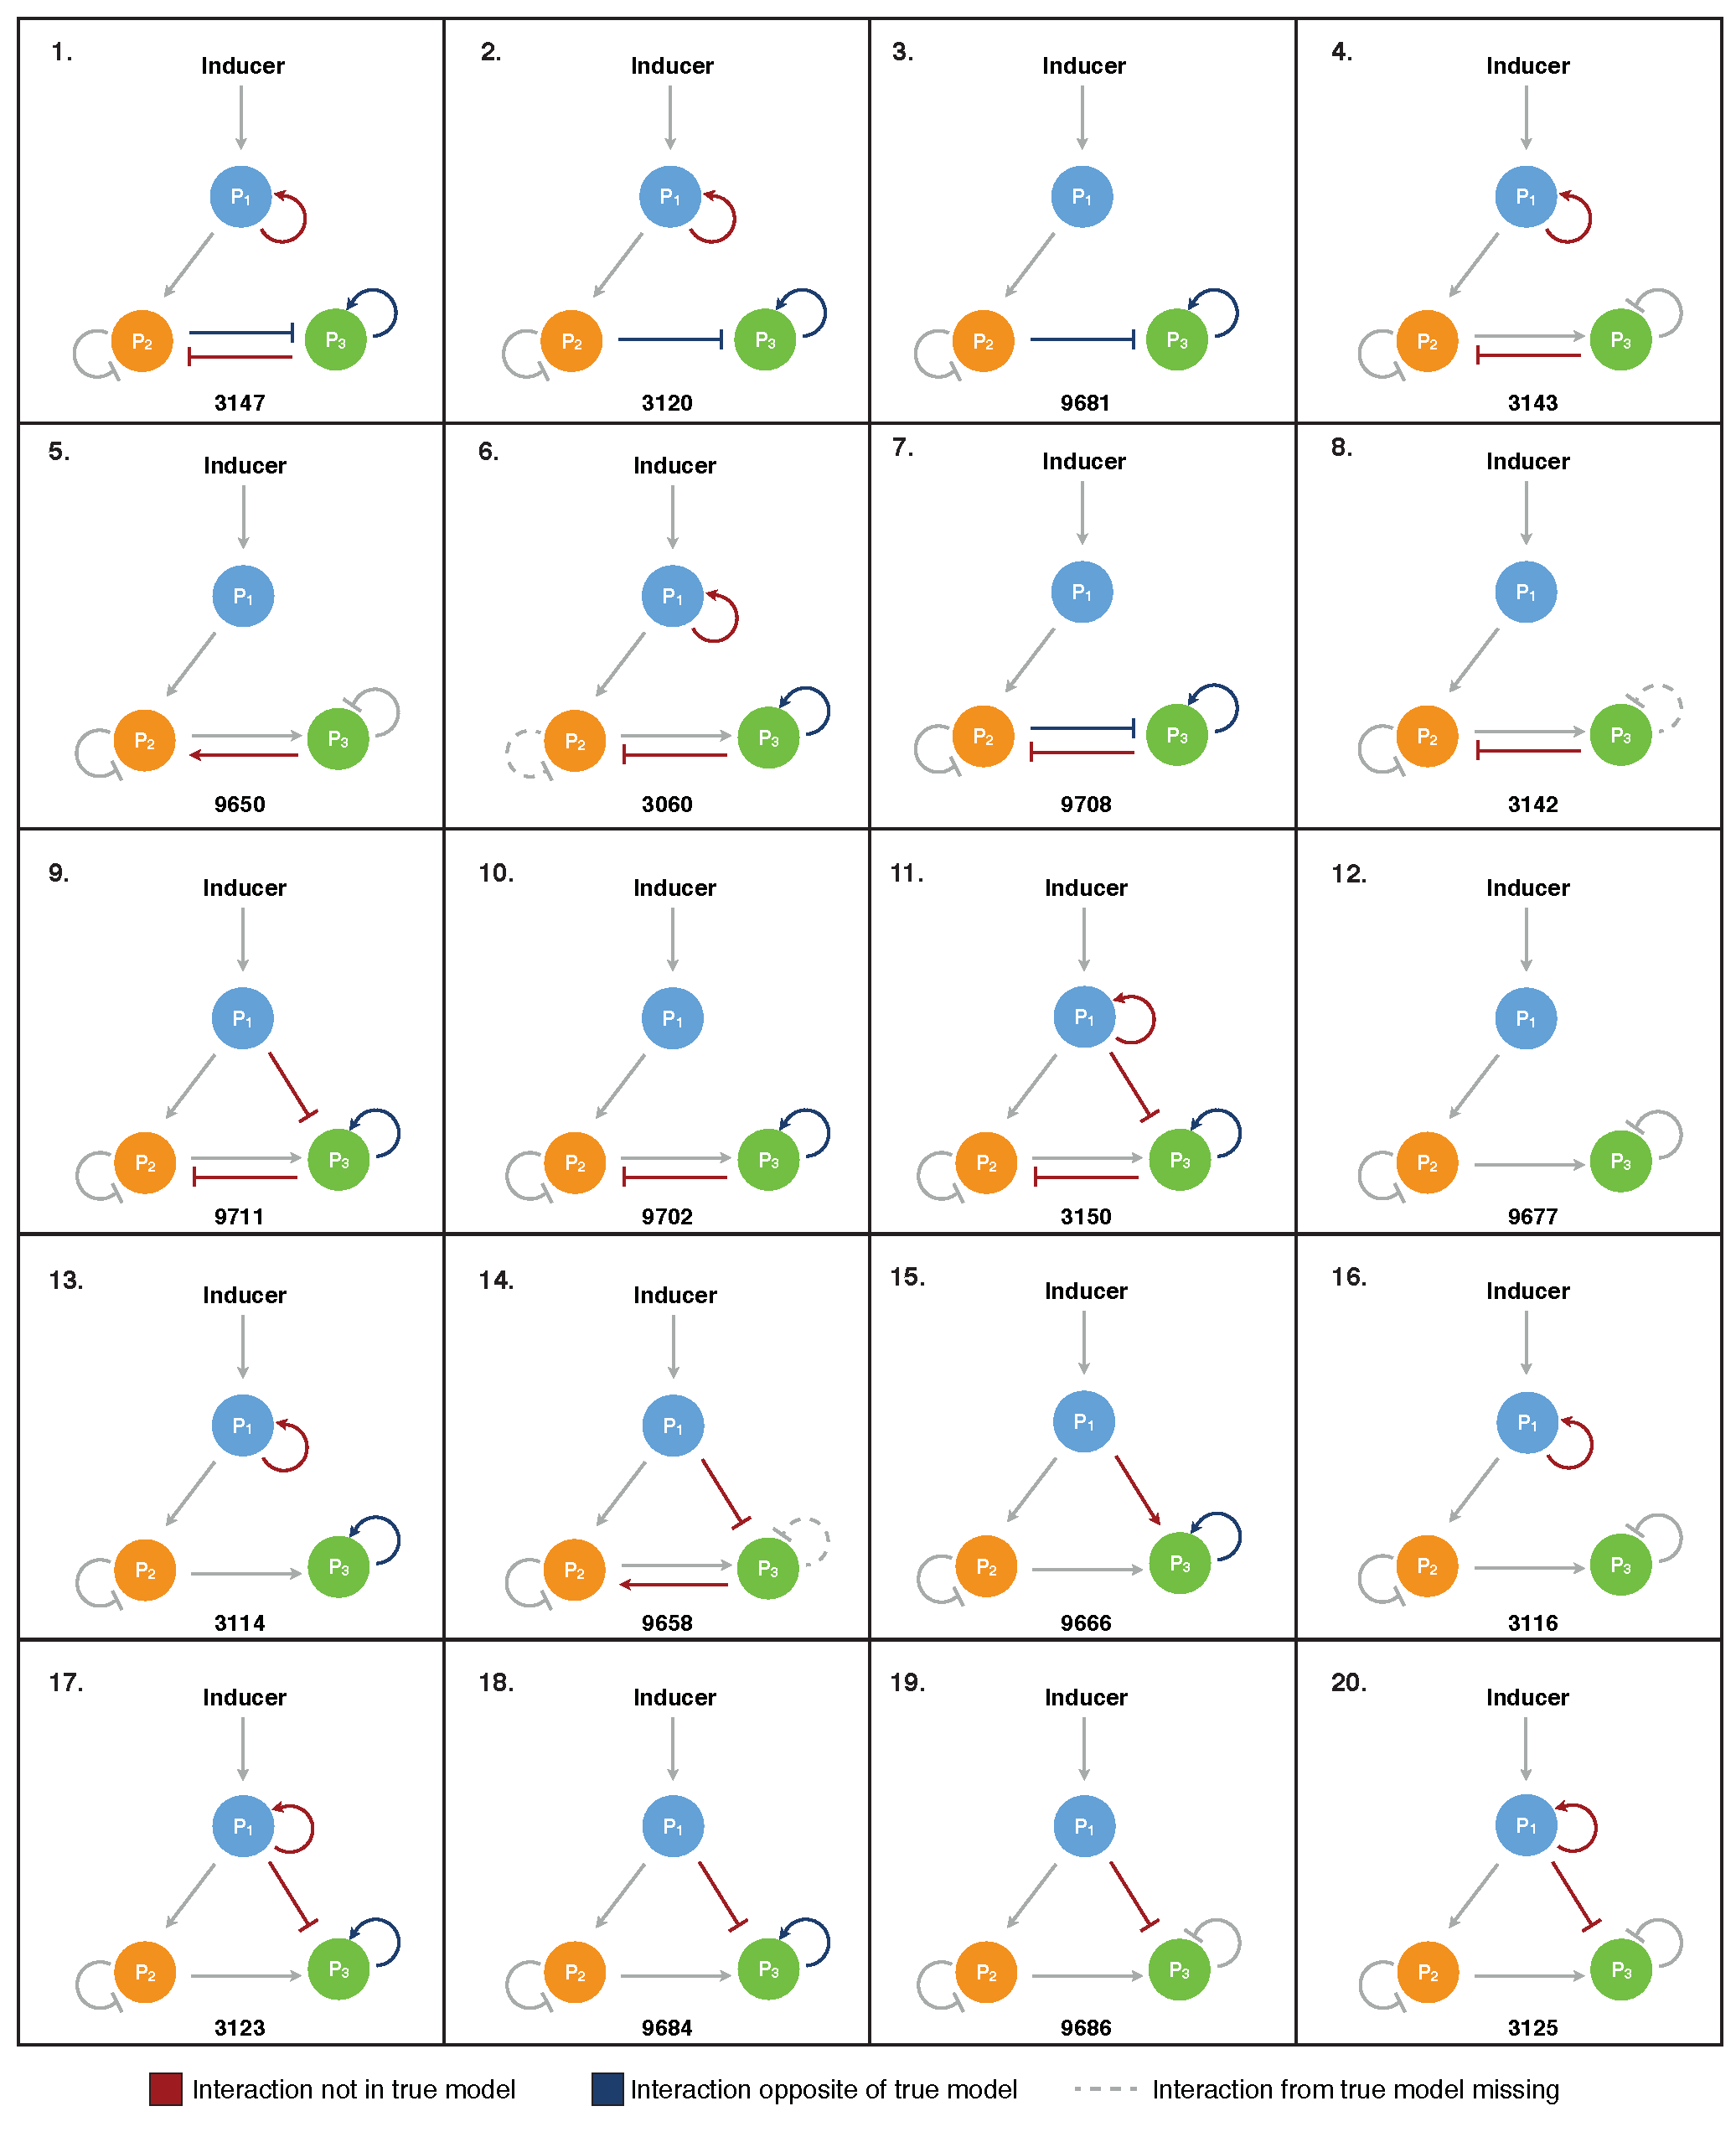
\includegraphics[width=1.0\textwidth]{./figs_chp3/3node_models_Table.pdf}
\caption{Structures of top 20 three protein node models. Models are arranged from lowest error (best fit) to highest error, with the true model at number 12. Red denotes interactions not in original model, blue denotes interactions that are opposite of the original model, and dotted lines denote interactions in true model that are missing in structure. Numbers (i.e. 3147) denote the specific model number out of the total 19683 structures.}
\label{fg:3node_models_Table}
\end{figure}

\clearpage

\begin{figure}\centering
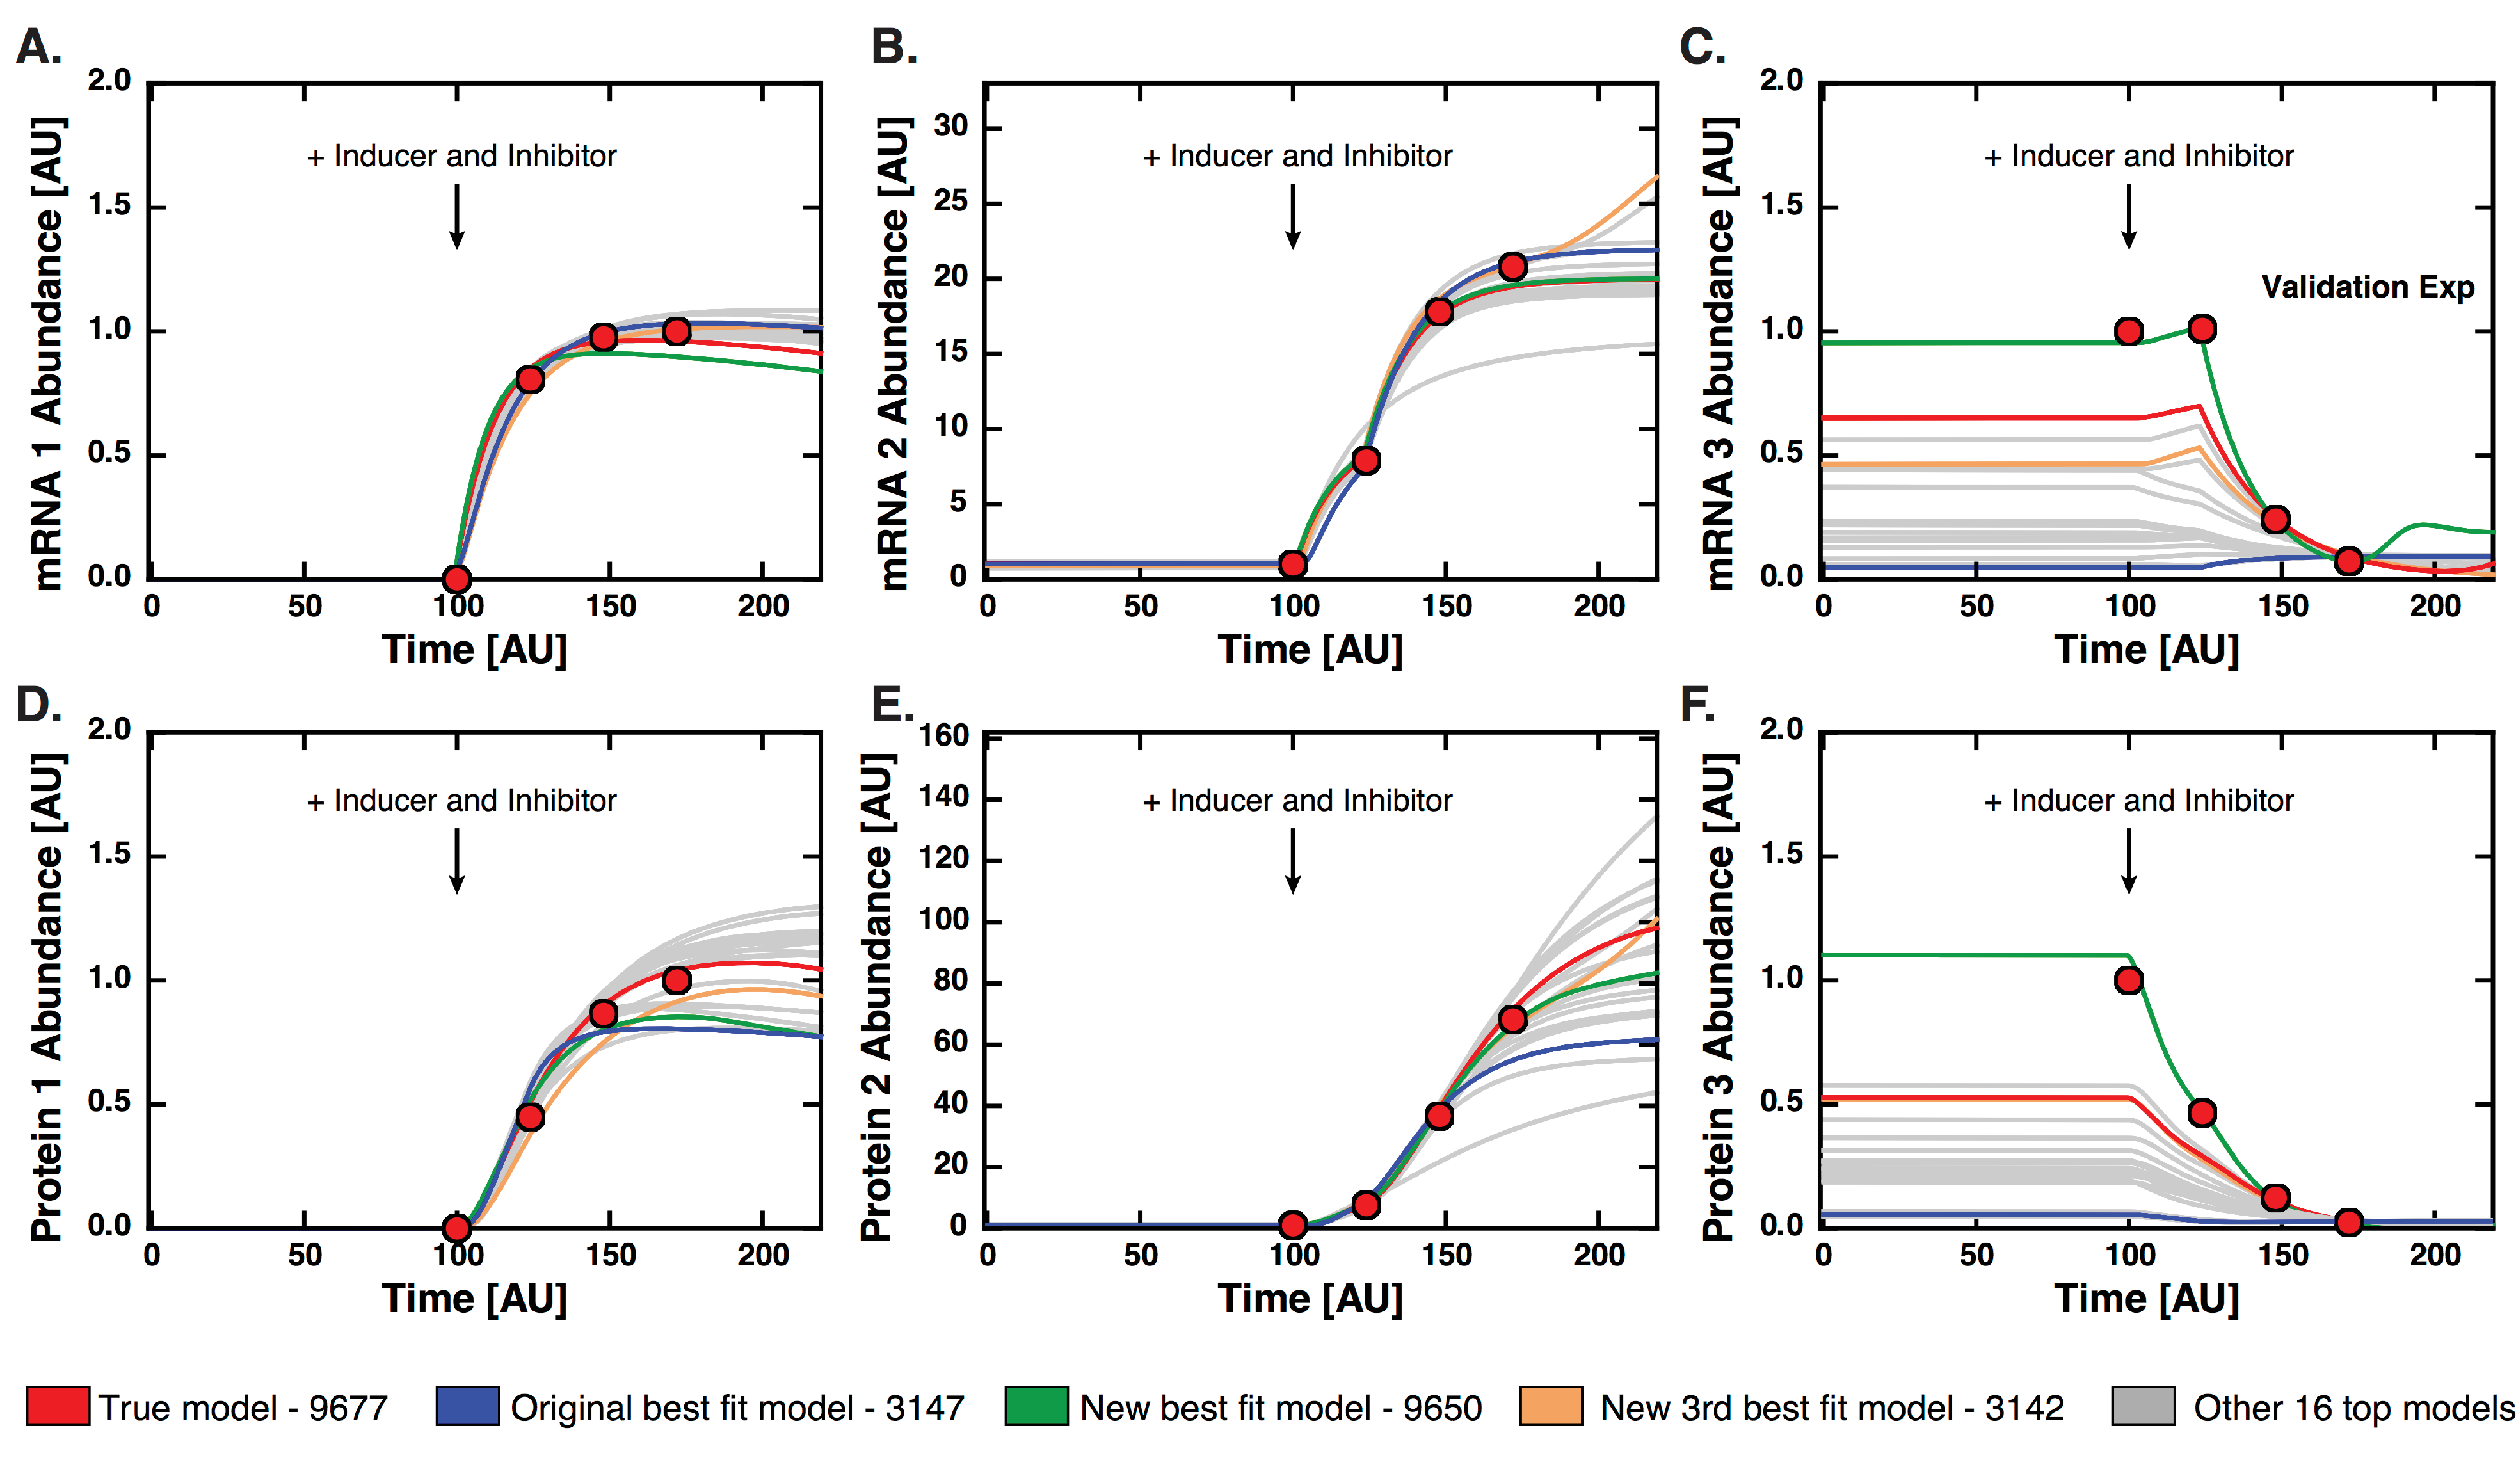
\includegraphics[width=1.0\textwidth]{./figs_chp3/Fig3_Top20_Exp2_2.pdf}
\caption{Experiment 2 results for the top 20 models with respective best parameter sets determined from particle swarm optimization. In experiment 2, inducer and an inhibitor for $P_{2}$ were added at Time = 100. $\bf{A, B.}$ Plots of mRNA concentration profiles for species 1 and 2 after inducer and inhibitor added at Time = 100. $\bf{C.}$ Plot of mRNA concentration profile for species 3 which was used for validation. $\bf{D, E, F.}$ Plots of protein concentration profiles for species 1, 2, and 3. Red dots denote synthetic experimental data used for fitting. Red lines represent the true model with new optimized parameters, blue denotes the best fitting model after experiment 1 (\ref{fg:3node_models}B), green denotes the new best fitting model, orange denotes the third best fit model, and the grey lines represent remaining top 18 models.}
\label{fg:Top20Models_Exp2}
\end{figure}

\clearpage

\begin{figure}\centering
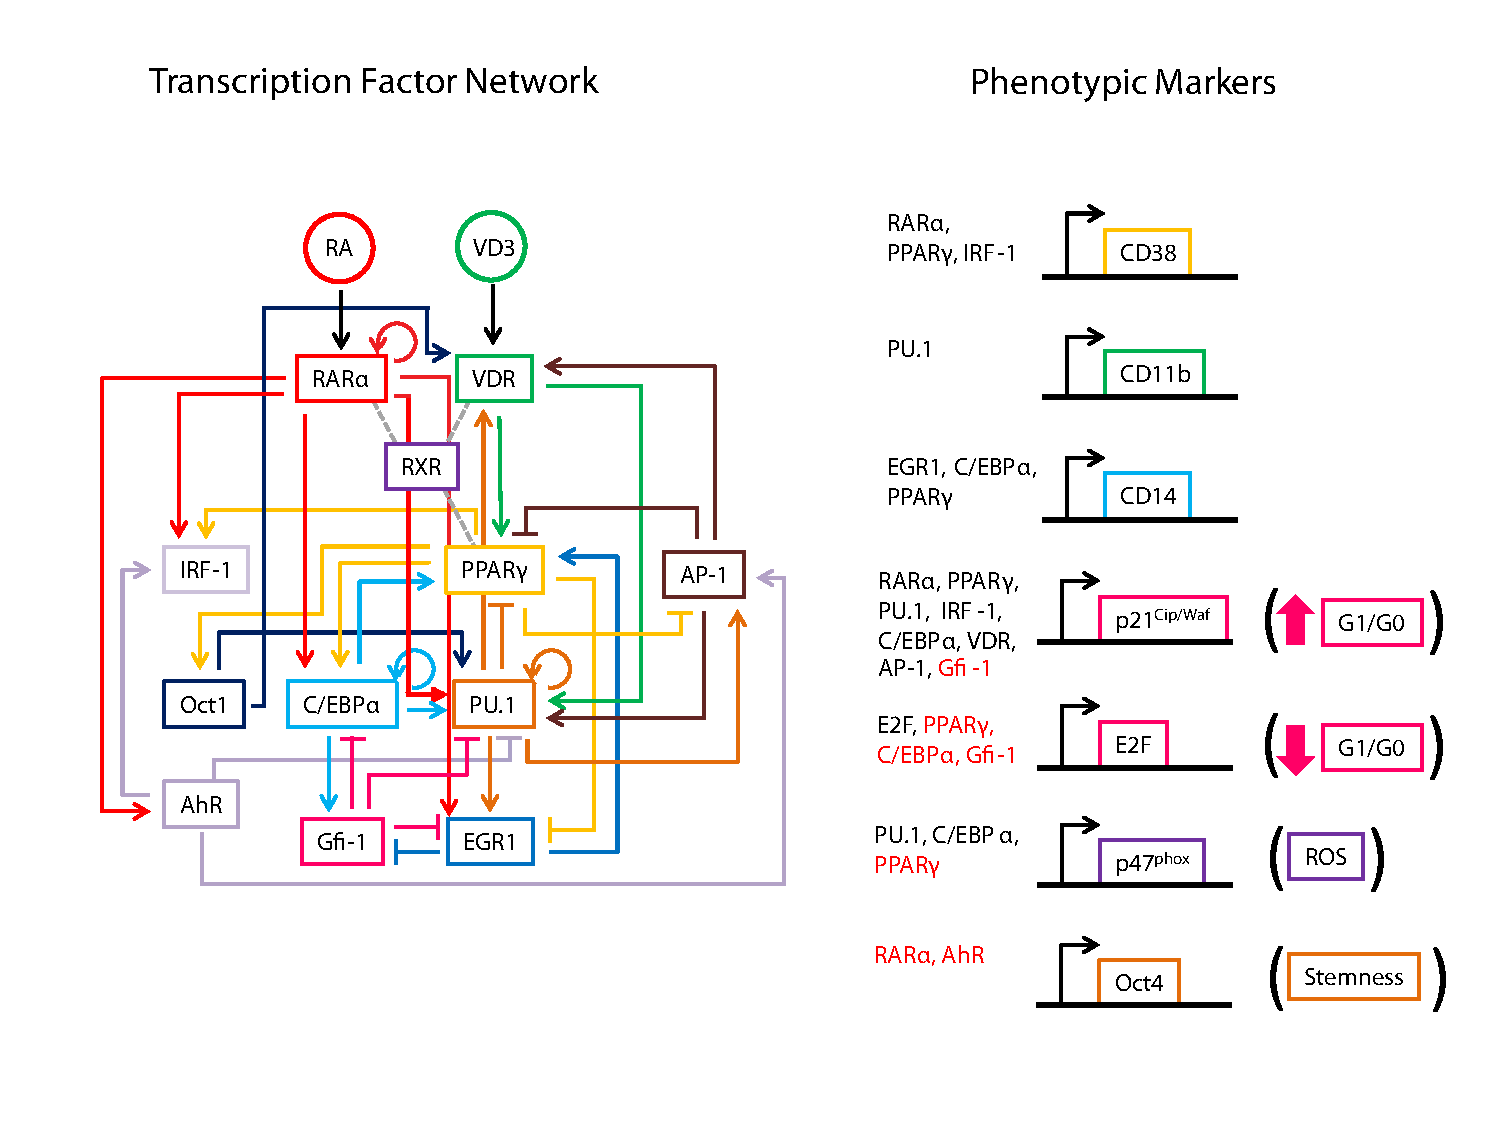
\includegraphics[width=1.0\textwidth]{./figs_chp3/TF_Network_new.pdf}
\caption{Initial myelomonocytic transcription factor network structure from literature sources. Figure shows interactions between protein nodes with arrows indicating transcriptional activation and lines indicating transcriptional repression. Phenotypic markers are shown on the right side, with black indicating activation and red repression. RXR (shown in the figure) was assumed to exist in an active form to dimerize with RAR$\alpha$, VDR, and PPAR$\gamma$ and was excluded in this network identification problem.}
\label{fg:Initial_TF_Network}
\end{figure}

\clearpage

\clearpage


\begin{center}
\renewcommand{\arraystretch}{0.8}
\tablefirsthead{
\hline
\rowcolor[gray]{0.8}\textbf{Transcription Factor}  & \textbf{General Effect} & \textbf{Target Gene} & \textbf{Reference(s)}  \\
\hline}
\topcaption{Initial myelomonocytic transcription factor network list with 
  transcription factor, effect, target gene, and reference}
\label{Leukemia_TF_Network}
\begin{scriptsize}
\begin{supertabular}{|p{3cm}|p{3cm}|p{3cm}|p{3cm}|}  
\hline											
RAR$\alpha$ &  upregulates & RAR$\alpha$ & \cite{Rishi1996} \\
RAR$\alpha$ &  upregulates & PU.1 & \cite{Mueller2006}\\
RAR$\alpha$ &  upregulates & C/EBP$\alpha$ & \cite{Friedman2007}\\
RAR$\alpha$ &  upregulates & IRF-1 & \cite{Luo2006}\\
RAR$\alpha$ &  represses & Oct4 & \cite{Sylvester1994}\\
RAR$\alpha$ &  upregulates & CD38 & \cite{Drach1994}\\
RAR$\alpha$ &  upregulates & p21 & \cite{Liu1996}\\
RAR$\alpha$ &  upregulates & AhR & \cite{Bunaciu2013}\\
RAR$\alpha$ &  upregulates & EGR1 & \cite{Balmer2002}\\
VDR &  upregulates & PPAR$\gamma$ & \cite{Dunlop2005}\\
VDR &  upregulates & PU.1 & \\
VDR &  upregulates & p21 & \cite{Liu1996a}\\
PPAR$\gamma$ &  upregulates & C/EBP$\alpha$ & \cite{Rosen2002}\\
PPAR$\gamma$ &  upregulates & IRF-1 & \cite{Varley2009}\\
PPAR$\gamma$ &  upregulates & Oct1 & \cite{Bruemmer2003}\\
PPAR$\gamma$ &  represses & AP-1 & \cite{Delerive1999}\\
PPAR$\gamma$ &  represses & E2F & \cite{Altiok1997}\\
PPAR$\gamma$ &  represses & EGR1 & \cite{Fei2011}\\
PPAR$\gamma$ &  upregulates & CD38 & \cite{Song2012}\\
PPAR$\gamma$ &  upregulates & CD14 & \cite{Szanto2005}\\
PPAR$\gamma$ &  upregulates & p21 & \cite{Han2004}\\
PPAR$\gamma$ &  represses & p47phox & \cite{Von-Knethen2002}\\
PU.1 &  represses & PPAR$\gamma$ & \cite{Dispirito2013}\\
PU.1 &  upregulates & PU.1 & \cite{Chen1995}\\
PU.1 &  upregulates & AP-1 & \cite{Steidl2006}\\
PU.1 &  upregulates & EGR1 & \cite{Laslo2006}\\
PU.1 &  upregulates & CD11b & \cite{Pahl1993}\\
PU.1 &  upregulates & p21 & \cite{Yuki2013}\\
PU.1 &  upregulates & p47phox & \cite{Li1999}\\
PU.1 &  upregulates & VDR & \cite{Gobel2009}\\
C/EBP$\alpha$ &  upregulates & PPAR$\gamma$ & \cite{Rosen2002}\\
C/EBP$\alpha$ &  upregulates & PU.1 & \cite{Dahl2003}\\
C/EBP$\alpha$ &  upregulates & C/EBP$\alpha$ & \cite{Timchenko1995}\\
C/EBP$\alpha$ &  upregulates & Gfi-1 & \cite{Lidonnici2010}\\
C/EBP$\alpha$ &  represses & E2F & \cite{DAlo2003}\\
C/EBP$\alpha$ &  upregulates & CD14 & \cite{Pan1999}\\
C/EBP$\alpha$ &  upregulates & p21 & \cite{Harris2001}\\
IRF-1 &  upregulates & CD38 & \cite{Bauvois1999}\\
IRF-1 &  upregulates & p21 & \cite{Passioura2005}\\
Gfi-1 &  represses & PU.1 & \cite{Dahl2007}\\
Gfi-1 &  represses & C/EBP$\alpha$ & \cite{Duan2003}\\
Gfi-1 &  represses & E2F & \cite{Duan2003}\\
Gfi-1 &  represses & EGR1 & \cite{Laslo2006}\\
Gfi-1 &  represses & p21 & \cite{Duan2003}\\
Oct1 &  upregulates & VDR & \cite{Liu1994}\\
Oct1 &  upregulates & PU.1 & \cite{Chen1996}\\
AP-1 &  upregulates & VDR &  \cite{Liu1994}\\
AP-1 &  represses & PPAR$\gamma$  & \cite{Delerive1999}\\
AP-1 &  upregulates & PU.1 &  \cite{Behre1999}\\
AP-1 &  upregulates & p21 &  \cite{Kardassis1999}\\
E2F &  upregulates & E2F & \cite{Johnson1994}\\
EGR1 &  upregulates & PPAR$\gamma$ & \cite{Fu2002}\\
EGR1 &  represses & Gfi-1 & \cite{Mak2011}\\
EGR1 &  upregulates & CD14 & \cite{Chen2004}\\
AhR &  upregulates & AP-1 & \cite{Suh2002}\\
AhR &  upregulates & IRF-1 & \cite{Shen2011}\\
AhR & represses & Oct4 & \cite{Bunaciu2011}\\
AhR & represses & PU.1 & \\

\hline
\end{supertabular}
\end{scriptsize}
\end{center}
%\end{document}







\clearpage

\begin{figure}\centering
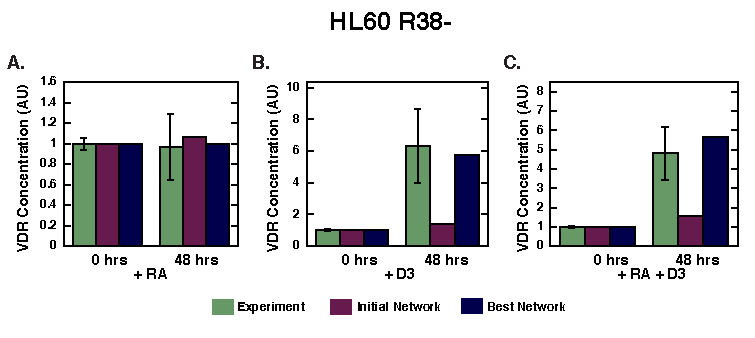
\includegraphics[width=1.0\textwidth]{./figs_chp3/Cell_Line_New/R38-HL60_Experiment_6.pdf}
\caption{Selected training results for the HL60 R38- cell line. $\bf{A., B., C.}$ Simulation and experimental results of change in VDR concentration due to RA, D3, and RA/D3 stimulus, respectively. Green denotes experimental data, pink denotes simulation data from the initial network, and blue denotes simulation data from the best network. The top parameter set is used, and error bars denote standard experimental error.}
\label{fg:R38-HL60_Experiment}
\end{figure}
\clearpage

\begin{figure}\centering
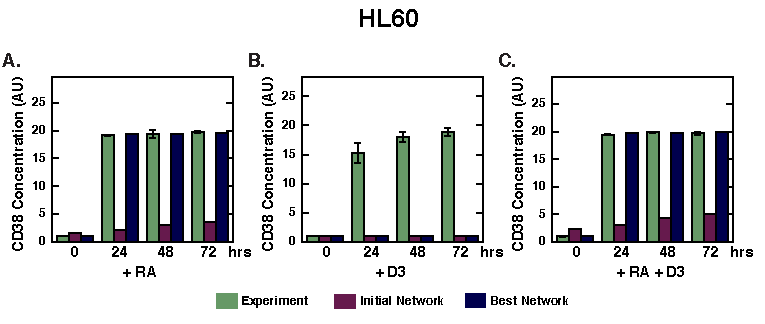
\includegraphics[width=1.0\textwidth]{./figs_chp3/Cell_Line_New/WTHL60_Experiment_10.pdf}
\caption{Selected training results for the HL60  cell line. $\bf{A., B., C.}$ Simulation and experimental results of change in cells expressing CD38 due to RA, D3, and RA/D3 stimulus, respectively. Green denotes experimental data, pink denotes simulation data from the initial network, and blue denotes simulation data from the best network. The top parameter set is used, and error bars denote standard experimental error.}
\label{fg:WTHL60_Experiment}
\end{figure}
\clearpage

\begin{figure}\centering
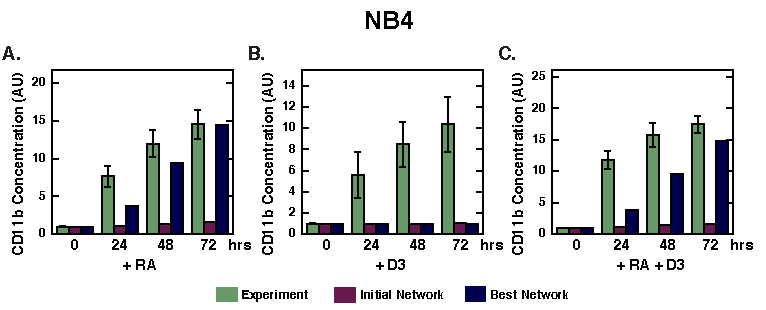
\includegraphics[width=1.0\textwidth]{./figs_chp3/Cell_Line_New/NB4_Experiment_11.pdf}
\caption{Selected training results for the NB4 cell line. $\bf{A., B., C.}$ Simulation and experimental results of change in CD11b concentration due to RA, D3, and RA/D3 stimulus, respectively. Green denotes experimental data, pink denotes simulation data from the initial network, and blue denotes simulation data from the best network. The top parameter set is used, and error bars denote standard experimental error.}
\label{fg:NB4_Experiment}
\end{figure}
\clearpage

\begin{figure}\centering
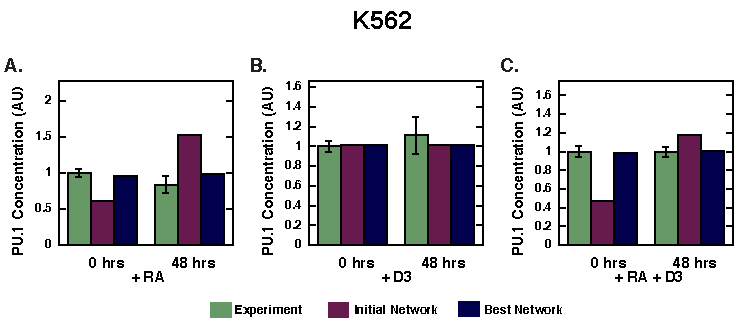
\includegraphics[width=1.0\textwidth]{./figs_chp3/Cell_Line_New/K562_Experiment_2.pdf}
\caption{Selected training results for the K562 cell line. $\bf{A., B., C.}$ Simulation and experimental results of change in PU.1 concentration due to RA, D3, and RA/D3 stimulus, respectively. Green denotes experimental data, pink denotes simulation data from the initial network, and blue denotes simulation data from the best network. The top parameter set is used, and error bars denote standard experimental error.}
\label{fg:K562_Experiment}
\end{figure}
\clearpage

% Supplemental figures -
% Set the S-
\renewcommand\thefigure{S\arabic{figure}}
\renewcommand\thetable{T\arabic{table}}
\renewcommand\thepage{S-\arabic{page}}
\renewcommand\theequation{S\arabic{equation}}

% Reset the counters -
\setcounter{equation}{0}
\setcounter{table}{0}
\setcounter{figure}{0}
\setcounter{page}{1}

\section*{Supplementary materials}

\clearpage

\begin{figure}\centering
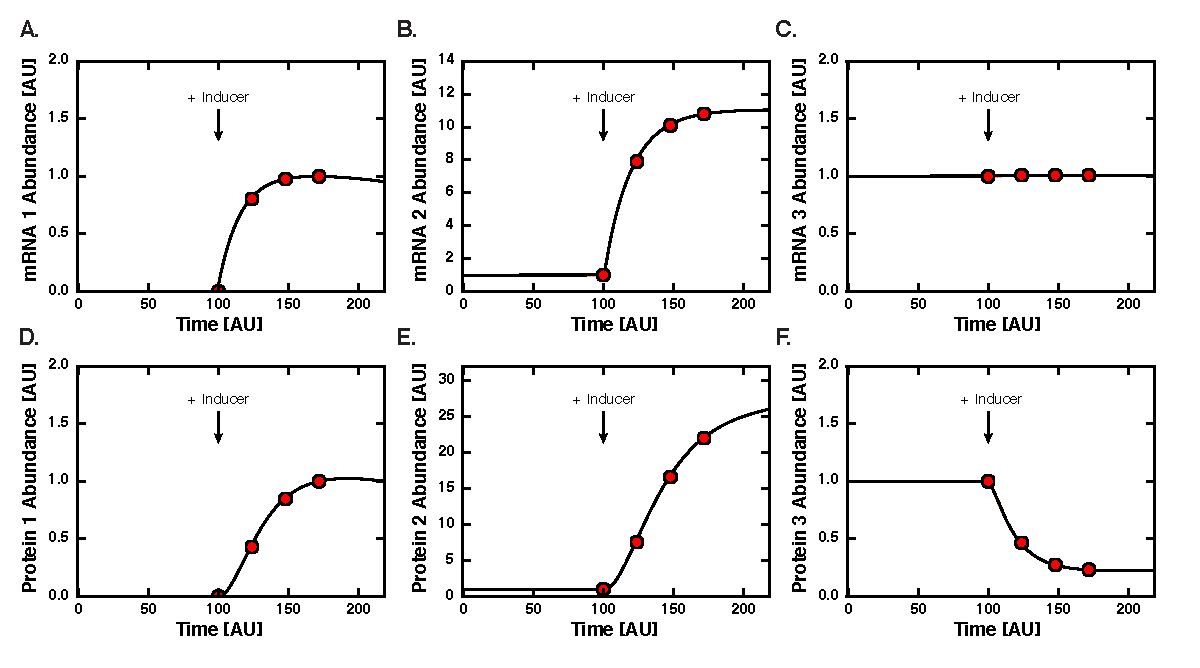
\includegraphics[width=1.0\textwidth]{./figs_chp3/True_Model_Simulation_9677.pdf}
\caption{Synthetic data running experiment 1 for true model of three node protein network. In experiment 1, inducer was added at Time = 100. $\bf{A, B, C.}$ Plots of mRNA concentration profiles for species 1, 2, and 3 after inducer added at Time = 100. $\bf{D, E, F.}$ Plots of protein concentration profiles for species 1, 2, and 3. Red dots denote data used for fitting (0, 24, 48, and 72 AU after stimulus).}
\label{fg:TrueModelData}
\end{figure}

\clearpage


\begin{center}
\tablefirsthead{
\hline
\rowcolor[gray]{0.8}\textbf{Objective \#}  & \textbf{Species} & \textbf{Experiment \#} & \textbf{Trial}  \\
\hline}
\topcaption{Training objective function list with 
  objective number, species measured, experiment and trials used in}
\label{3_node_objective}
\begin{scriptsize}
\begin{supertabular}{|p{2cm}|p{3cm}|p{3cm}|p{3cm}|}  
\hline											
O1 &  $mRNA_{1}$ & Exp1 & 1, 2 \\
O2 &  $mRNA_{2}$ & Exp1 & 1, 2 \\
O3 &  $mRNA_{3}$ & Exp1 & 1, 2 \\
O4 &  $P_{2}$ & Exp1 & 1, 2 \\
O5 &  $P_{3}$ & Exp1 & 1, 2 \\
O6 &  $mRNA_{1}$ & Exp2 & 2 \\
O7 &  $mRNA_{2}$ & Exp2 & 2 \\
O8 &  $P_{1}$ & Exp2 & 2 \\
O9 &  $P_{2}$ & Exp2 & 2 \\
O10 &  $P_{3}$ & Exp2 & 2 \\
O11 &  $mRNA_{1}$ & Exp3 & 2 \\
O12 &  $mRNA_{2}$ & Exp3 & 2 \\
O13 &  $mRNA_{3}$ & Exp3 & 2 \\
O14 &  $P_{1}$ & Exp3 & 2 \\
O15 &  $P_{3}$ & Exp3 & 2 \\
\hline
\end{supertabular}
\end{scriptsize}
\end{center}
%\end{document}

\vspace{10mm}


\begin{center}
\tablefirsthead{
\hline
\rowcolor[gray]{0.8}\textbf{Prediction \#}  & \textbf{Species} & \textbf{Experiment \#} & \textbf{Trial}  \\
\hline}
\topcaption{Prediction function list with 
  prediction number, species measured, experiment and trials used in}
\label{3_node_prediction}
\begin{scriptsize}
\begin{supertabular}{|p{2cm}|p{3cm}|p{3cm}|p{3cm}|}  
\hline											
P1 &  $P_{1}$ & Exp1 & 1, 2 \\
P2 &  $mRNA_{3}$  & Exp2 & 2 \\
P3 &  $P_{2}$ & Exp2 & 2 \\
\hline
\end{supertabular}
\end{scriptsize}
\end{center}
%\end{document}

\clearpage

\clearpage


\begin{center}
\tablefirsthead{
\hline
\rowcolor[gray]{0.8}\textbf{Experiment \#}  & \textbf{Stimulus} & \textbf{Training Species} & \textbf{Validation Species}  \\
\hline}
\topcaption{Experiment list with 
  stimulus, species for training, and species for validation}
\label{exp_table}
\begin{scriptsize}
\begin{supertabular}{|p{2cm}|p{5cm}|p{3cm}|p{3cm}|}  
\hline											
1 &  At t = 100, Inducer = +10 & $mRNA_{1}$, $mRNA_{2}$, $mRNA_{3}$, $P_{2}$, $P_{3}$ & $P_{1}$ \\
2 &  At t = 100, Inducer = +10 and inhibit binding of protein 2 &  $mRNA_{1}$, $mRNA_{2}$, $P_{1}$, $P_{2}$, $P_{3}$ & $mRNA_{3}$\\
3 &  At t = 100, 124, 148, 172, 196, Inducer = +1 &  $mRNA_{1}$, $mRNA_{2}$, $mRNA_{3}$, $P_{1}$, $P_{3}$ & $P_{2}$\\
%4 &  At t = 100, Inducer = +10 and inhibit binding of protein 3 &  $mRNA_{2}$, $mRNA_{3}$, $P_{1}$, $P_{2}$, $P_{3}$ & $mRNA_{1}$\\
%5 &  At t = 100, Inducer = +10 and inhibit binding of protein 1 &  $mRNA_{1}$, $mRNA_{2}$, $mRNA_{3}$, $P_{1}$, $P_{2}$ & $P_{3}$ \\
%6 &  At t = 100,  inhibit binding of protein 3 &  $mRNA_{1}$, $mRNA_{2}$, $mRNA_{3}$, $P_{2}$, $P_{3}$ & $P_{1}$ \\
\hline
\end{supertabular}
\end{scriptsize}
\end{center}
%\end{document}

\clearpage

\clearpage


\begin{center}
\tablefirsthead{
\hline
\rowcolor[gray]{0.8}\textbf{Objective \#}  & \textbf{Species Measured} & \textbf{Stimulus} & \textbf{Time Point (hrs)}  \\
\hline}
\topcaption{Training objective function list with 
  objective number, species measured, stimulus, and time points. The same 39 objective functions were used for all cell lines with data from \cite{Jensen2015}.}
\label{Leukemia_TF_objective}
\begin{scriptsize}
\begin{supertabular}{|p{2cm}|p{3cm}|p{3cm}|p{3cm}|}  
\hline											
O1 & C/EBP$\alpha$ & 1 $\mu$M RA & 48 \\
O2 &  PU.1 & 1 $\mu$M RA & 48 \\
O3 &  EGR1 & 1 $\mu$M RA & 48 \\
O4 &  Gfi-1 & 1 $\mu$M RA & 48 \\
O5 &  RAR$\alpha$ & 1 $\mu$M RA & 48 \\
O6 &  VDR & 1 $\mu$M RA & 48 \\
O7 &  IRF-1 & 1 $\mu$M RA & 48 \\
O8 &  Oct4 & 1 $\mu$M RA & 48 \\
O9 &  AhR & 1 $\mu$M RA & 48 \\
O10 & CD38 & 1 $\mu$M RA & 24, 48, 72 \\
O11 &  CD11b & 1 $\mu$M RA & 24, 48, 72 \\
O12 &  CD14 & 1 $\mu$M RA & 24, 48, 72 \\
O13 &  G1/G0 & 1 $\mu$M RA & 24, 48, 72 \\
O14 & C/EBP$\alpha$ & 0.5 $\mu$M VD3 & 48 \\
O15 &  PU.1 & 0.5 $\mu$M VD3 & 48 \\
O16 &  EGR1 & 0.5 $\mu$M VD3 & 48 \\
O17 &  Gfi-1 & 0.5 $\mu$M VD3 & 48 \\
O18 &  RAR$\alpha$ & 0.5 $\mu$M VD3 & 48 \\
O19 &  VDR & 0.5 $\mu$M VD3 & 48 \\
O20 &  IRF-1 & 0.5 $\mu$M VD3 & 48 \\
O21 &  Oct4 & 0.5 $\mu$M VD3 & 48 \\
O22 &  AhR & 0.5 $\mu$M VD3 & 48 \\
O23 & CD38 & 0.5 $\mu$M VD3 & 24, 48, 72 \\
O24 &  CD11b & 0.5 $\mu$M VD3 & 24, 48, 72 \\
O25 &  CD14 & 0.5 $\mu$M VD3 & 24, 48, 72 \\
O26 &  G1/G0 & 0.5 $\mu$M VD3 & 24, 48, 72 \\
O27 & C/EBP$\alpha$ & 1 $\mu$M RA, 0.5 $\mu$M VD3 & 48 \\
O28 &  PU.1 & 1 $\mu$M RA, 0.5 $\mu$M VD3 & 48 \\
O29 &  EGR1 & 1 $\mu$M RA, 0.5 $\mu$M VD3 & 48 \\
O30 &  Gfi-1 & 1 $\mu$M RA, 0.5 $\mu$M VD3 & 48 \\
O31 &  RAR$\alpha$ & 1 $\mu$M RA, 0.5 $\mu$M VD3 & 48 \\
O32 &  VDR & 1 $\mu$M RA, 0.5 $\mu$M VD3 & 48 \\
O33 &  IRF-1 & 1 $\mu$M RA, 0.5 $\mu$M VD3 & 48 \\
O34 &  Oct4 & 1 $\mu$M RA, 0.5 $\mu$M VD3 & 48 \\
O35 &  AhR & 1 $\mu$M RA, 0.5 $\mu$M VD3 & 48 \\
O36 & CD38 & 1 $\mu$M RA, 0.5 $\mu$M VD3 & 24, 48, 72 \\
O37 &  CD11b & 1 $\mu$M RA, 0.5 $\mu$M VD3 & 24, 48, 72 \\
O38 &  CD14 & 1 $\mu$M RA, 0.5 $\mu$M VD3 & 24, 48, 72 \\
O39 &  G1/G0 & 1 $\mu$M RA, 0.5 $\mu$M VD3 & 24, 48, 72 \\

\hline
\end{supertabular}
\end{scriptsize}
\end{center}
%\end{document}

\clearpage

\begin{figure}\centering
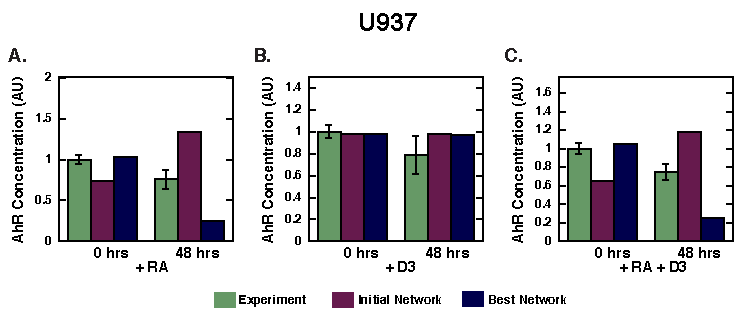
\includegraphics[width=1.0\textwidth]{./figs_chp3/Cell_Line_New/U937_Experiment_9.pdf}
\caption{Selected training results for the U937 cell line. $\bf{A., B., C.}$ Simulation and experimental results of change in AhR concentration due to RA, D3, and RA/D3 stimulus, respectively. Green denotes experimental data, pink denotes simulation data from the initial network, and blue denotes simulation data from the best network. The top parameter set is used, and error bars denote standard experimental error.}
\label{fg:U937_Experiment}
\end{figure}
\clearpage

\begin{figure}\centering
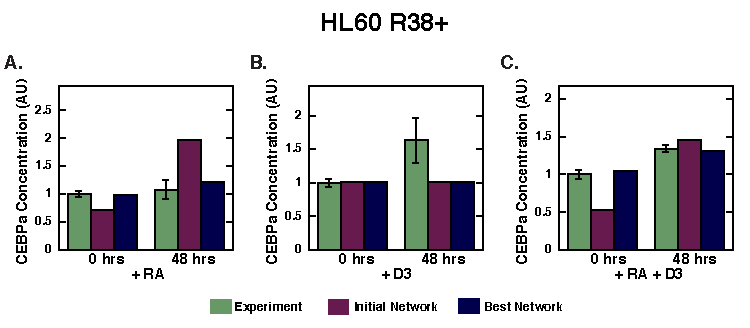
\includegraphics[width=1.0\textwidth]{./figs_chp3/Cell_Line_New/R38+HL60_Experiment_1.pdf}
\caption{Selected training results for the HL60 R38+ cell line. $\bf{A., B., C.}$ Simulation and experimental results of change in C/EBP$\alpha$ concentration due to RA, D3, and RA/D3 stimulus, respectively. Green denotes experimental data, pink denotes simulation data from the initial network, and blue denotes simulation data from the best network. The top parameter set is used, and error bars denote standard experimental error.}
\label{fg:R38+HL60_Experiment}
\end{figure}
\clearpage


\clearpage


\begin{center}
\renewcommand{\arraystretch}{0.8}
\tablefirsthead{
\hline
\rowcolor[gray]{0.8}\textbf{Edge Number}  & \textbf{Action} & \textbf{
Transcription Factor} &  \textbf{General Effect} &  \textbf{Target Gene} & \textbf{Reference(s)}  \\
\hline}
\topcaption{Model Updates for K562 cell line with edge number, action, transcription factor, general effect, target gene, and new references}
\label{K562_Model}
\begin{scriptsize}
\begin{supertabular}{|p{2 cm}|p{2cm}|p{3cm}|p{2.5cm}|p{2cm}|p{1.5cm}|}  
\hline	
6 &  deleted & RAR$\alpha$   & upregulates &  AhR & \\
7 &  deleted & RAR$\alpha$   & upregulates &  C/EBP$\alpha$ & \\
8 &  added & RAR$\alpha$   & represses & Gfi-1 & \\ 
9 &  deleted & RAR$\alpha$   & upregulates &  EGR1 & \\
11 &  added & RAR$\alpha$   & represses &  AP-1  & \cite{Benkoussa2002} \\
14 &  added & RAR$\alpha$   & represses &  CD14 & \\
20 &  added & VDR  & represses &  VDR & \\
22 &  added & VDR  & upregulates &  IRF-1 & \\
23 &  added & VDR  & represses &  Oct1 & \\
25 &  added & VDR  & represses &  C/EBP$\alpha$ & \\
27 &  added & VDR  & represses &  EGR1 & \\
31 &  added & VDR  & represses &  CD11b & \\
32 &  added & VDR  & upregulates &  CD14 & \cite{Sadeghi2006} \\
34 &  added & VDR  & upregulates &  E2F & \\
38 &  added & PPAR$\gamma$  & upregulates &  VDR & \\
49 &  added & PPAR$\gamma$  & represses &  CD11b & \\
50 &  deleted & PPAR$\gamma$  & upregulates &  CD14 & \\
52 &  deleted & PPAR$\gamma$  & represses &  E2F & \\
56 &  added & IRF-1  & represses &  VDR & \\
59 &  added & IRF-1  & upregulates &  Oct1 & \\
61 &  added & IRF-1  & upregulates &  C/EBP$\alpha$ & \\
63 &  added & IRF-1  & upregulates &  EGR1 & \\
64 &  added & IRF-1  & represses &  PU.1 & \\
65 &  added & IRF-1  & represses &  AP-1 & \\
67 &  added & IRF-1  & upregulates &  CD11b & \\
70 &  added & IRF-1  & upregulates &  E2F & \\
76 &  added & Oct1  & represses &  IRF-1 & \\
77 &  added & Oct1  & represses &  Oct1 & \\
78 &  added & Oct1  & upregulates &  AhR & \\
82 &  deleted & Oct1  & upregulates &  PU.1 & \\
83 &  added & Oct1  & upregulates &  AP-1 & \cite{Ullman1993} \\
86 &  added & Oct1  & upregulates &  CD14 & \\
87 &  added & Oct1  & represses &  p21 & \\
88 &  added & Oct1  & upregulates &  E2F & \\
89 &  added & Oct1  & represses &  p47phox & \\
90 &  added & Oct1  & represses &  Oct4 & \\
92 &  added & AhR  & upregulates &  VDR & \\
97 &  added & AhR  & represses &  C/EBP$\alpha$ & \\
99 &  added & AhR  & upregulates &  EGR1 & \cite{Martinez2004} \\
102 &  added & AhR  & represses &  CD38 & \\
107 &  added & AhR  & upregulates &  p47phox & \\
110 &  added & C/EBP$\alpha$  & represses &  VDR & \\
117 &  added & C/EBP$\alpha$  & represses &  EGR1 & \cite{Hasemann2014}\\
118 &  deleted & C/EBP$\alpha$  & upregulates &  PU.1 & \\
121 &  added & C/EBP$\alpha$  & upregulates &  CD11b & \\
122 &  switched &  C/EBP$\alpha$  & represses &  CD14 & \\
128 &  added & Gfi-1  & represses &  VDR & \\
129 &  added & Gfi-1  & represses &  PPAR$\gamma$ & \\
130 &  added & Gfi-1  & represses &  IRF-1 & \\
134 &  added & Gfi-1  & represses &  Gfi-1 & \cite{Doan2004}\\
141 &  deleted & Gfi-1  & represses &  p21 & \\
144 &  added & Gfi-1  & represses &  Oct4 & \\
146 &  added & EGR1  & represses &  VDR & \\
147 &  switched &  EGR1  & represses &  PPAR$\gamma$ & \\
150 &  added & EGR1  & upregulates &  AhR & \\
155 &  added & EGR1  & upregulates &  AP-1 & \\
157 &  added & EGR1  & upregulates &  CD11b & \\
162 &  added & EGR1  & represses &  Oct4 & \\
164 &  deleted & PU.1  & upregulates &  VDR & \\
168 &  added & PU.1  & represses &  AhR & \\
169 &  added & PU.1  & represses &  C/EBP$\alpha$ & \\
170 &  added & PU.1  & upregulates &  Gfi-1 & \cite{Laslo2006}\\
173 &  deleted & PU.1  & upregulates &  AP-1 & \\
174 &  added & PU.1  & represses &  CD38 & \\
177 &  deleted & PU.1  & upregulates &  p21 & \\
178 &  added & PU.1  & upregulates &  E2F & \\
179 &  switched &  PU.1  & represses &  p47phox & \\
180 &  added & PU.1  & upregulates &  Oct4 & \\
182 &  switched &  AP-1  & represses &  VDR & \\
184 &  added & AP-1  & upregulates &  IRF-1 & \\
187 &  deleted & AP-1  & represses &  C/EBP$\alpha$ & \\
188 &  added & AP-1  & upregulates &  Gfi-1 & \\
189 &  added & AP-1  & upregulates &  EGR1 & \\
195 &  switched &  AP-1  & represses &  p21 & \\
198 &  added & AP-1  & represses &  Oct4 & \\
255 &  added & p21  & represses &  PPAR$\gamma$ & \\
257 &  added & p21  & upregulates &  Oct1 & \\
258 &  added & p21  & represses &  AhR & \\
259 &  added & p21  & represses &  C/EBP$\alpha$ & \\
260 &  added & p21  & represses &  Gfi-1 & \\
263 &  added & p21  & upregulates &  AP-1 & \\
265 &  added & p21  & represses &  CD11b & \\
274 &  added & E2F  & upregulates &  IRF-1 & \\
275 &  added & E2F  & represses &  Oct1 & \\
276 &  added & E2F  & represses &  AhR & \\
277 &  added & E2F  & represses &  C/EBP$\alpha$ &\cite{Zaragoza2010} \\
279 &  added & E2F  & upregulates &  EGR1 & \\
280 &  added & E2F  & represses &  PU.1 & \\
281 &  added & E2F  & represses &  AP-1 & \\
282 &  added & E2F  & upregulates &  CD38 & \\
283 &  added & E2F  & represses &  CD11b & \\
284 &  added & E2F  & represses &  CD14 & \\
286 &  switched &  E2F  & represses &  E2F & \\
287 &  added & E2F  & upregulates &  p47phox & \\
313 &  added & Oct4  & upregulates &  C/EBP$\alpha$ & \\
318 &  added & Oct4  & represses &  CD38 & \\
319 &  added & Oct4  & upregulates &  CD11b & \\
320 &  added & Oct4  & upregulates &  CD14 & \\
322 &  added & Oct4  & represses &  E2F & \\
324 &  added & Oct4  & represses &  Oct4 & \\

\hline
\end{supertabular}
\end{scriptsize}
\end{center}
%\end{document}







\clearpage

\clearpage


\begin{center}
\renewcommand{\arraystretch}{0.8}
\tablefirsthead{
\hline
\rowcolor[gray]{0.8}\textbf{Edge Number}  & \textbf{Action} & \textbf{
Transcription Factor} &  \textbf{General Effect} &  \textbf{Target Gene} & \textbf{Reference(s)}  \\
\hline}
\topcaption{Model Updates for NB4 cell line with edge number, action, transcription factor, general effect, target gene, and new references}
\label{NB4_Model}
\begin{scriptsize}
\begin{supertabular}{|p{2 cm}|p{2cm}|p{3cm}|p{2.5cm}|p{2cm}|p{1.5cm}|}  
\hline	

3 &  added &  RAR$\alpha$ & represses &  PPAR$\gamma$ & \\
6 &  deleted &  RAR$\alpha$ & upregulates &  AhR & \\
9 &  switched &  RAR$\alpha$ & represses &  EGR1 & \\
10 &  switched &  RAR$\alpha$ & represses &  PU.1 & \\
11 &  added &  RAR$\alpha$ & upregulates &  AP-1 & \\
13 &  added &  RAR$\alpha$ & upregulates &  CD11b & \\
16 &  added &  RAR$\alpha$ & represses &  E2F & \\
17 &  added &  RAR$\alpha$ & upregulates &  p47phox & \cite{Balmer2002}\\
18 &  switched &  RAR$\alpha$ & upregulates &  Oct4 &  \cite{Ben-Shushan1995}\\
22 &  added &  VDR  & represses &  IRF-1 & \\
24 &  added &  VDR  & upregulates &  AhR & \\
26 &  added &  VDR  & upregulates &  Gfi-1 & \\
36 &  added &  VDR  & upregulates &  Oct4 & \\
38 &  added &  PPAR$\gamma$  & upregulates &  VDR & \\
39 &  added &  PPAR$\gamma$ & represses &  PPAR$\gamma$ & \\ 
45 &  deleted &  PPAR$\gamma$ & represses &  EGR1 & \\
46 &  added &  PPAR$\gamma$ & represses &  PU.1 & \\
58 &  added &  IRF-1  & represses &  IRF-1 & \\
60 &  added &  IRF-1  & represses &  AhR & \\
62 &  added &  IRF-1  & upregulates &  Gfi-1 & \\
63 &  added &  IRF-1  & upregulates &  EGR1 & \\
66 &  switched &  IRF-1  & represses &  CD38 & \\
70 &  added &  IRF-1  & represses &  E2F & \\
72 &  added &  IRF-1  & upregulates &  Oct4 & \\
76 &  added &  Oct1  & upregulates &  IRF-1 & \\
77 &  added &  Oct1  & upregulates &  Oct1 & \cite{Pankratova2003}\\
81 &  added &  Oct1  & represses &  EGR1 & \\
83 &  added &  Oct1  & upregulates &  AP-1 & \cite{Ullman1993}\\
86 &  added &  Oct1  & represses &  CD14 & \\
89 &  added &  Oct1  & upregulates &  p47phox & \\ 
90 &  added &  Oct1  & represses &  Oct4 & \\
92 &  added &  AhR  & upregulates &  VDR & \\
96 &  added &  AhR  & upregulates &  AhR & \\
98 &  added &  AhR  & upregulates &  Gfi-1 & \\
100 &  switched &  AhR  & upregulates &  PU.1 & \\
103 &  added &  AhR  & upregulates &  CD11b & \\
104 &  added &  AhR  & represses &  CD14 & \\
106 &  added &  AhR  & represses &  E2F & \cite{Marlowe2004}\\
110 &  added &  C/EBP$\alpha$  & upregulates &  VDR & \\
111 &  switched &  C/EBP$\alpha$  & represses &  PPAR$\gamma$ & \\
113 &  added &  C/EBP$\alpha$  & upregulates &  Oct1 & \\
114 &  added &  C/EBP$\alpha$  & upregulates &  AhR & \\
116 &  deleted &  C/EBP$\alpha$  & upregulates &  Gfi-1 & \\
117 &  added &  C/EBP$\alpha$  & represses &  EGR1 & \cite{Hasemann2014}\\
118 &  deleted &  C/EBP$\alpha$  & upregulates &  PU.1 & \\
122 &  switched &  C/EBP$\alpha$  & represses &  CD14 & \\
124 &  switched &  C/EBP$\alpha$  & upregulates &  E2F & \\
129 &  added &  Gfi-1  & represses &  PPAR$\gamma$  & \\
133 &  deleted &  Gfi-1  & represses &  C/EBP$\alpha$ & \\
138 &  added &  Gfi-1  & represses &  CD38 & \\
143 &  added &  Gfi-1  & represses &  p47phox & \\
152 &  switched &  EGR1  & upregulates &  Gfi-1 & \\
156 &  added &  EGR1  & represses &  CD38 & \\
157 &  added &  EGR1  & upregulates &  CD11b & \\
167 &  added &  PU.1  & represses &  Oct1 & \\
172 &  switched &  PU.1  & represses &  PU.1 & \\
175 &  deleted &  PU.1  & upregulates &  CD11b & \\
178 &  added &  PU.1  & upregulates &  E2F & \\
180 &  added &  PU.1  & represses &  Oct4 & \\
182 &  deleted &  AP-1  & upregulates &  VDR & \\
186 &  added &  AP-1  & upregulates &  AhR & \\
188 &  added &  AP-1  & represses &  Gfi-1 & \\
189 &  added &  AP-1  & upregulates &  EGR1 & \\
190 &  deleted &  AP-1  & upregulates &  PU.1 & \\
191 &  added &  AP-1  & represses &  AP-1 & \\
193 &  added &  AP-1  & upregulates &  CD11b & \\
196 &  added &  AP-1  & upregulates &  E2F & \cite{Shen2008}\\
197 &  added &  AP-1  & represses &  p47phox & \\
254 &  added &  p21  & upregulates &  VDR & \\
255 &  added &  p21  & upregulates &  PPAR$\gamma$ & \\
256 &  added &  p21  & represses &  IRF-1 & \\
260 &  added &  p21  & upregulates &  Gfi-1 & \\
262 &  added &  p21  & upregulates &  PU.1 & \\
265 &  added &  p21  & upregulates &  CD11b & \\
268 &  added &  p21  & upregulates &  E2F & \\
272 &  added &  E2F  & upregulates &  VDR & \\
273 &  added &  E2F  & represses &  PPAR$\gamma$ & \\
274 &  added &  E2F  & upregulates &  IRF-1 & \\
276 &  added &  E2F  & upregulates &  AhR & \\
281 &  added &  E2F  & upregulates &  AP-1 & \\
283 &  added &  E2F  & upregulates &  CD11b & \\
284 &  added &  E2F  & upregulates &  CD14 & \\
286 &  switched &  E2F  & represses &  E2F & \\
288 &  added &  E2F  & represses &  Oct4 & \\
309 &  added &  Oct4  & upregulates &  PPAR$\gamma$ & \\
310 &  added &  Oct4  & represses &  IRF-1 & \\
312 &  added &  Oct4  & upregulates &  AhR & \\ 
314 &  added &  Oct4  & upregulates &  Gfi-1 & \\
317 &  added &  Oct4  & represses &  AP-1 & \\
320 &  added &  Oct4  & upregulates &  CD14 & \\

\hline
\end{supertabular}
\end{scriptsize}
\end{center}
%\end{document}







\clearpage

\clearpage


\begin{center}
\renewcommand{\arraystretch}{0.8}
\tablefirsthead{
\hline
\rowcolor[gray]{0.8}\textbf{Edge Number}  & \textbf{Action} & \textbf{
Transcription Factor} &  \textbf{General Effect} &  \textbf{Target Gene} & \textbf{Reference(s)}  \\
\hline}
\topcaption{Model Updates for WT-HL60 cell line with edge number, action, transcription factor, general effect, target gene, and new references}
\label{WTHL60_Model}
\begin{scriptsize}
\begin{supertabular}{|p{2 cm}|p{2cm}|p{3cm}|p{2.5cm}|p{2cm}|p{1.5cm}|}  
\hline

2 &  added &  RAR$\alpha$  & represses & VDR & \\
3 &  added &  RAR$\alpha$  & upregulates &  PPAR$\gamma$ & \\
5 &  added &  RAR$\alpha$  & represses & Oct1 & \\
6 &  switched &  RAR$\alpha$  & represses & AhR & \\
7 &  switched &  RAR$\alpha$  & represses &C/EBP$\alpha$ & \\
8 &  added &  RAR$\alpha$  & represses & Gfi-1 & \\
13 &  added &  RAR$\alpha$  & upregulates &  CD11b & \\
14 &  added &  RAR$\alpha$  & represses & CD14 & \\
17 &  added &  RAR$\alpha$  & upregulates &  p47phox & \cite{Balmer2002}\\
21 &  deleted &  VDR  & upregulates &  PPAR$\gamma$ & \\
27 &  added &  VDR  & represses & EGR1 & \\
34 &  added &  VDR  & represses & E2F & \\
38 &  added &  PPAR$\gamma$  & upregulates &  VDR & \\
39 &  added &  PPAR$\gamma$  & represses & PPAR$\gamma$ & \\
40 &  switched &  PPAR$\gamma$  & represses & IRF-1 & \\
42 &  added &  PPAR$\gamma$  & upregulates &  AhR & \\
45 &  switched &  PPAR$\gamma$  & upregulates &  EGR1 & \\
48 &  deleted &  PPAR$\gamma$  & upregulates &  CD38 & \\
49 &  added &  PPAR$\gamma$  & upregulates &  CD11b & \\
50 &  switched &  PPAR$\gamma$  & represses & CD14 & \\
53 &  deleted &  PPAR$\gamma$  & represses & p47phox & \\
56 &  added &  IRF-1  & upregulates &  VDR & \\
66 &  switched &  IRF-1  & represses & CD38 & \\
68 &  added &  IRF-1  & represses & CD14 & \\
70 &  added &  IRF-1  & represses & E2F & \\
74 &  switched &  Oct1  & represses & VDR & \\
78 &  added &  Oct1  & upregulates &  AhR & \\
79 &  added &  Oct1  & upregulates & C/EBP$\alpha$ & \\
83 &  added &  Oct1  & upregulates &  AP1 & \cite{Ullman1993}\\
85 &  added &  Oct1  & upregulates &  CD11b & \\
87 &  added &  Oct1  & upregulates &  p21 & \\
88 &  added &  Oct1  & represses & E2F & \\
89 &  added &  Oct1  & represses & p47phox & \\
95 &  added &  AhR  & upregulates &  Oct1 & \\
96 &  added &  AhR  & represses & AhR & \\
100 &  switched &  AhR  & upregulates &  PU.1 & \\
101 &  deleted &  AhR  & upregulates &  AP1 & \\
103 &  added &  AhR  & represses & CD11b & \\
104 &  added &  AhR  & upregulates &  CD14 & \\
106 &  added &  AhR  & upregulates &  E2F & \cite{Marlowe2004}\\
110 &  added & C/EBP$\alpha$ & upregulates &  VDR & \\
113 &  added & C/EBP$\alpha$ & represses & Oct1 & \\
118 &  switched & C/EBP$\alpha$ & represses & PU.1 & \\
119 &  added & C/EBP$\alpha$ & upregulates &  AP1 & \\
122 &  deleted & C/EBP$\alpha$ & upregulates &  CD14 & \\
123 &  deleted & C/EBP$\alpha$ & upregulates &  p21 & \\
125 &  added & C/EBP$\alpha$ & upregulates &  p47phox & \\
126 &  added & C/EBP$\alpha$ & represses & Oct4 & \\
136 &  deleted &  Gfi-1  & represses & PU.1 & \\
141 &  deleted &  Gfi-1  & represses & p21 & \\
142 &  deleted &  Gfi-1  & represses & E2F & \\
143 &  added &  Gfi-1  & represses & p47phox & \\
148 &  added &  EGR1  & upregulates &  IRF-1 & \\
149 &  added &  EGR1  & represses & Oct1 & \\
151 &  added &  EGR1  & represses &C/EBP$\alpha$ & \\
155 &  added &  EGR1  & represses & AP1 & \\
158 &  deleted &  EGR1  & upregulates &  CD14 & \\
159 &  added &  EGR1  & upregulates &  p21 & \\
164 &  deleted &  PU.1  & upregulates &  VDR & \\
165 &  deleted &  PU.1  & represses & PPAR$\gamma$ & \\
167 &  added &  PU.1  & represses & Oct1 & \\
174 &  added &  PU.1  & upregulates &  CD38 & \\
176 &  added &  PU.1  & represses & CD14 & \\
179 &  deleted &  PU.1  & upregulates &  p47phox & \\
181 &  added &  AP1  & upregulates &  RAR$\alpha$ & \\
182 &  deleted &  AP1  & upregulates &  VDR & \\
183 &  added &  AP1  & represses & PPAR$\gamma$ & \cite{Wang2002}\\
185 &  added &  AP1  & represses & Oct1 & \\
191 &  added &  AP1  & represses & AP1 & \\
193 &  added &  AP1  & upregulates &  CD11b & \\
254 &  added &  p21  & upregulates &  VDR & \\
257 &  added &  p21  & upregulates &  Oct1 & \\
258 &  added &  p21  & upregulates &  AhR & \\
261 &  added &  p21  & represses & EGR1 & \\
262 &  added &  p21  & upregulates &  PU.1 & \\
264 &  added &  p21  & upregulates &  CD38 & \\
270 &  added &  p21  & upregulates &  Oct4 & \\
272 &  added &  E2F  & represses & VDR & \\
273 &  added &  E2F  & represses & PPAR$\gamma$ & \\
274 &  added &  E2F  & upregulates &  IRF-1 & \\
275 &  added &  E2F  & represses & Oct1 & \\
276 &  added &  E2F  & upregulates &  AhR & \\
281 &  added &  E2F  & represses & AP1 & \\
283 &  added &  E2F  & represses & CD11b & \\
312 &  added &  Oct4  & represses & AhR & \\
314 &  added &  Oct4  & upregulates &  Gfi-1 & \\
316 &  added &  Oct4  & upregulates &  PU.1 & \\
317 &  added &  Oct4  & represses & AP1 & \\
319 &  added &  Oct4  & represses & CD11b & \\
320 &  added &  Oct4  & represses & CD14 & \\
323 &  added &  Oct4  & upregulates &  p47phox & \\	

\hline
\end{supertabular}
\end{scriptsize}
\end{center}
%\end{document}







\clearpage

\clearpage


\begin{center}
\renewcommand{\arraystretch}{0.8}
\tablefirsthead{
\hline
\rowcolor[gray]{0.8}\textbf{Edge Number}  & \textbf{Action} & \textbf{
Transcription Factor} &  \textbf{General Effect} &  \textbf{Target Gene} & \textbf{Reference(s)}  \\
\hline}
\topcaption{Model Updates for HL60 R38+ cell line with edge number, action, transcription factor, general effect, target gene, and new references}
\label{HL60+R38_Model}
\begin{scriptsize}
\begin{supertabular}{|p{2 cm}|p{2cm}|p{3cm}|p{2.5cm}|p{2cm}|p{1.5cm}|}  
\hline

10 &  deleted &  RAR$\alpha$   & upregulates &  PU.1 & \\
13 &  added &  RAR$\alpha$   & upregulates &  CD11b & \\
16 &  added &  RAR$\alpha$   & upregulates &  E2F & \\
18 &  deleted &  RAR$\alpha$   & upregulates &  Oct4 & \\
21 &  switched &  VDR  & upregulates &  PPAR$\gamma$ & \\
22 &  added &  VDR  & upregulates &  IRF-1 & \\
23 &  added &  VDR  & upregulates &  Oct1 & \\
29 &  added &  VDR  & upregulates &  AP1 & \cite{Wu2007}\\
31 &  added &  VDR  & upregulates &  CD11b & \\
32 &  added &  VDR  & upregulates &  CD14 & \cite{Sadeghi2006}\\
36 &  added &  VDR  & upregulates &  Oct4 & \\
40 &  deleted &  PPAR$\gamma$  & upregulates &  IRF-1 & \\
44 &  added &  PPAR$\gamma$  & upregulates &  Gfi-1 & \\
52 &  deleted &  PPAR$\gamma$  & upregulates &  E2F & \\
54 &  added &  PPAR$\gamma$  & upregulates &  Oct4 & \\
59 &  added &  IRF-1  & upregulates &  Oct1 & \\
62 &  added &  IRF-1  & upregulates &  Gfi-1 & \\
63 &  added &  IRF-1  & upregulates &  EGR1 & \\
64 &  added &  IRF-1  & upregulates &  PU.1 & \\
69 &  deleted &  IRF-1  & upregulates &  p21 & \\
71 &  added &  IRF-1  & upregulates &  p47phox & \\
76 &  added &  Oct1  & upregulates &  IRF-1 & \\
81 &  added &  Oct1  & upregulates &  EGR1 & \\
82 &  switched &  Oct1  & upregulates &  PU.1 & \\
88 &  added &  Oct1  & upregulates &  E2F & \\
90 &  added &  Oct1  & upregulates &  Oct4 & \\
94 &  deleted &  AhR  & upregulates &  IRF-1 & \\
99 &  added &  AhR  & upregulates &  EGR1 & \cite{Martinez2004}\\
100 &  deleted &  AhR  & upregulates &  PU.1 & \\
102 &  added &  AhR  & upregulates &  CD38 & \\
105 &  added &  AhR  & upregulates &  p21 & \\
107 &  added &  AhR  & upregulates &  p47phox & \\
111 &  deleted &  C/EBP$\alpha$  & upregulates &  PPAR$\gamma$ & \\
112 &  added &  C/EBP$\alpha$  & upregulates &  IRF-1 & \\
114 &  added &  C/EBP$\alpha$  & upregulates &  AhR & \\
116 &  switched &  C/EBP$\alpha$  & upregulates &  Gfi-1 & \\
117 &  added &  C/EBP$\alpha$  & upregulates &  EGR1 & \\
118 &  switched &  C/EBP$\alpha$  & upregulates &  PU.1 & \\
119 &  added &  C/EBP$\alpha$  & upregulates &  AP1 & \\
120 &  added &  C/EBP$\alpha$  & upregulates &  CD38 & \\
125 &  added &  C/EBP$\alpha$  & upregulates &  p47phox & \\
131 &  added &  Gfi-1  & upregulates &  Oct1 & \\
132 &  added &  Gfi-1  & upregulates &  AhR & \\
133 &  deleted &  Gfi-1  & upregulates &  C/EBP$\alpha$ & \\
135 &  deleted &  Gfi-1  & upregulates &  EGR1 & \\
139 &  added &  Gfi-1  & upregulates &  CD11b & \\
142 &  deleted &  Gfi-1  & upregulates &  E2F & \\
150 &  added &  EGR1  & upregulates &  AhR & \\
152 &  deleted &  EGR1  & upregulates &  Gfi-1 & \\
154 &  added &  EGR1  & upregulates &  PU.1 & \cite{Friedman2002}\\
156 &  added &  EGR1  & upregulates &  CD38 & \\
161 &  added &  EGR1  & upregulates &  p47phox & \\
165 &  switched &  PU.1  & upregulates &  PPAR$\gamma$ & \\
167 &  added &  PU.1  & upregulates &  Oct1 & \\
170 &  added &  PU.1  & upregulates &  Gfi-1 & \\
173 &  switched &  PU.1  & upregulates &  AP1 & \\
175 &  deleted &  PU.1  & upregulates &  CD11b & \\
179 &  deleted &  PU.1  & upregulates &  p47phox & \\
183 &  added &  AP1  & upregulates &  PPAR$\gamma$ & \cite{Wang2002}\\
188 &  added &  AP1  & upregulates &  Gfi-1 & \\
192 &  added &  AP1  & upregulates &  CD38 & \\
195 &  deleted &  AP1  & upregulates &  p21 & \\
256 &  added &  p21  & upregulates &  IRF-1 & \\
261 &  added &  p21  & upregulates &  EGR1 & \\
266 &  added &  p21  & upregulates &  CD14 & \\
269 &  added &  p21  & upregulates &  p47phox & \\
270 &  added &  p21  & upregulates &  Oct4 & \\
274 &  added &  E2F  & upregulates &  IRF-1 & \\
279 &  added &  E2F  & upregulates &  EGR1 & \\
310 &  added &  Oct4  & upregulates &  IRF-1 & \\
312 &  added &  Oct4  & upregulates &  AhR & \\
315 &  added &  Oct4  & upregulates &  EGR1 & \\
318 &  added &  Oct4  & upregulates &  CD38 & \\
320 &  added &  Oct4  & upregulates &  CD14	& \\ 

\hline
\end{supertabular}
\end{scriptsize}
\end{center}
%\end{document}







\clearpage

\clearpage


\begin{center}
\renewcommand{\arraystretch}{0.8}
\tablefirsthead{
\hline
\rowcolor[gray]{0.8}\textbf{Edge Number}  & \textbf{Action} & \textbf{
Transcription Factor} &  \textbf{General Effect} &  \textbf{Target Gene} & \textbf{Reference(s)}  \\
\hline}
\topcaption{Model Updates for HL60 R38- cell line with edge number, action, transcription factor, general effect, target gene, and new references}
\label{HL60-R38_Model}
\begin{scriptsize}
\begin{supertabular}{|p{2 cm}|p{2cm}|p{3cm}|p{2.5cm}|p{2cm}|p{1.5cm}|}  
\hline

7 &  deleted &  RAR$\alpha$  & upregulates &  C/EBP$\alpha$ & \\
9 &  switched &  RAR$\alpha$  & represses &  EGR1 & \\
14 &  added &  RAR$\alpha$  & represses &  CD14 & \\
16 &  added &  RAR$\alpha$  & upregulates &  E2F & \\
21 &  deleted &  VDR  & upregulates &  PPAR$\gamma$ & \\
25 &  added &  VDR  & represses &  C/EBP$\alpha$ & \\
26 &  added &  VDR  & represses &  Gfi-1 & \\
29 &  added &  VDR  & represses &  AP-1 & \cite{Wu2007}\\
40 &  deleted &  PPAR$\gamma$  & upregulates &  IRF-1 & \\
41 &  switched &  PPAR$\gamma$  & represses &  Oct1 & \\
43 &  switched &  PPAR$\gamma$  & represses &  C/EBP$\alpha$ & \\
46 &  added &  PPAR$\gamma$  & upregulates &  PU.1 & \\
47 &  switched &  PPAR$\gamma$  & upregulates &  AP-1 & \\
49 &  added &  PPAR$\gamma$  & upregulates &  CD11b & \\
57 &  added &  IRF-1  & upregulates &  PPAR$\gamma$ & \\
58 &  added &  IRF-1  & upregulates &  IRF-1 & \\
62 &  added &  IRF-1  & represses &  Gfi-1 & \\
63 &  added &  IRF-1  & represses &  EGR1 & \\
64 &  added &  IRF-1  & upregulates &  PU.1 & \\
65 &  added &  IRF-1  & represses &  AP-1 & \\
66 &  deleted &  IRF-1  & upregulates &  CD38 & \\
67 &  added &  IRF-1  & upregulates &  CD11b & \\
70 &  added &  IRF-1  & upregulates &  E2F & \\
71 &  added &  IRF-1  & represses &  p47phox & \\
73 &  added &  Oct1  & represses &  RAR$\alpha$ & \cite{Kakizawa1999}\\
75 &  added &  Oct1  & upregulates &  PPAR$\gamma$ & \\
78 &  added &  Oct1  & represses &  AhR & \\
83 &  added &  Oct1  & represses &  AP-1 & \cite{Ullman1993}\\
87 &  added &  Oct1  & upregulates &  p21 & \\
89 &  added &  Oct1  & represses &  p47phox & \\
91 &  added &  AhR  & upregulates &  RAR$\alpha$ & \cite{Widerak2006}\\
93 &  added &  AhR  & upregulates &  PPAR$\gamma$ & \\
94 &  deleted &  AhR  & upregulates &  IRF-1 & \\
100 &  deleted &  AhR  & represses &  PU.1 & \\
101 &  switched &  AhR  & represses &  AP-1 & \\
104 &  added &  AhR  & represses &  CD14 & \\
105 &  added &  AhR  & represses &  p21 & \\
109 &  added &  C/EBP$\alpha$  & upregulates &  RAR$\alpha$ & \\
110 &  added &  C/EBP$\alpha$  & upregulates &  VDR & \\
111 &  deleted &  C/EBP$\alpha$  & upregulates &  PPAR$\gamma$ & \\
114 &  added &  C/EBP$\alpha$  & upregulates &  AhR & \\
116 &  deleted &  C/EBP$\alpha$  & upregulates &  Gfi-1 & \\
118 &  deleted &  C/EBP$\alpha$  & upregulates &  PU.1 & \\
119 &  added &  C/EBP$\alpha$  & upregulates &  AP-1 & \\
124 &  deleted &  C/EBP$\alpha$  & represses &  E2F & \\
125 &  added &  C/EBP$\alpha$  & upregulates &  p47phox & \\
132 &  added &  Gfi-1  & represses &  AhR & \\
133 &  deleted &  Gfi-1  & represses &  C/EBP$\alpha$ & \\
139 &  added &  Gfi-1  & represses &  CD11b & \\
140 &  added &  Gfi-1  & represses &  CD14 & \\
141 &  deleted &  Gfi-1  & represses &  p21 & \\
146 &  added &  EGR1  & represses &  VDR & \\
150 &  added &  EGR1  & upregulates &  AhR & \\
156 &  added &  EGR1  & upregulates &  CD38 & \\
158 &  deleted &  EGR1  & upregulates &  CD14 & \\
160 &  added &  EGR1  & represses &  E2F & \\
162 &  added &  EGR1  & upregulates &  Oct4 & \\
176 &  added &  PU.1  & upregulates &  CD14 & \\
178 &  added &  PU.1  & represses &  E2F & \\
180 &  added &  PU.1  & upregulates &  Oct4 & \\
194 &  added &  AP-1  & represses &  CD14 & \\
195 &  switched &  AP-1  & represses &  p21 & \\
256 &  added &  p21  & upregulates &  IRF-1 & \\
263 &  added &  p21  & upregulates &  AP-1 & \\
266 &  added &  p21  & represses &  CD14 & \\
269 &  added &  p21  & represses &  p47phox & \\
272 &  added &  E2F  & represses &  VDR & \\
275 &  added &  E2F  & represses &  Oct1 & \\
279 &  added &  E2F  & represses &  EGR1 & \\
283 &  added &  E2F  & upregulates &  CD11b & \\
309 &  added &  Oct4  & upregulates &  PPAR$\gamma$ & \\
317 &  added &  Oct4  & represses &  AP-1 & \\
318 &  added &  Oct4  & upregulates &  CD38 & \\
319 &  added &  Oct4  & upregulates &  CD11b & \\
321 &  added &  Oct4  & upregulates &  p21 & \\
323 &  added &  Oct4  & upregulates &  p47phox & \\

\hline
\end{supertabular}
\end{scriptsize}
\end{center}
%\end{document}







\clearpage

\clearpage


\begin{center}
\renewcommand{\arraystretch}{0.8}
\tablefirsthead{
\hline
\rowcolor[gray]{0.8}\textbf{Edge Number}  & \textbf{Action} & \textbf{
Transcription Factor} &  \textbf{General Effect} &  \textbf{Target Gene} & \textbf{Reference(s)}  \\
\hline}
\topcaption{Model Updates for U937 cell line with edge number, action, transcription factor, general effect, target gene, and new references}
\label{U937_Model}
\begin{scriptsize}
\begin{supertabular}{|p{2 cm}|p{2cm}|p{3cm}|p{2.5cm}|p{2cm}|p{1.5cm}|}  
\hline	

2 &  added & RAR$\alpha$  & upregulates &  VDR & \\
13 &  added & RAR$\alpha$  & upregulates &  CD11b & \\
14 &  added & RAR$\alpha$  & represses &  CD14 & \\
17 &  added & RAR$\alpha$  & upregulates &  p47phox & \\
27 &  added & VDR  & upregulates &  EGR1 & \\
36 &  added & VDR  & upregulates &  Oct4 & \\
44 &  added & PPAR$\gamma$  & upregulates &  Gfi-1 & \\
48 &  deleted &  PPAR$\gamma$  & upregulates &  CD38 & \\
62 &  added & IRF-1  & upregulates &  Gfi-1 & \\
71 &  added & IRF-1  & represses &  p47phox & \\
72 &  added & IRF-1  & represses &  Oct4 & \\
73 &  added & Oct1  & upregulates &  RAR$\alpha$ & \cite{Kakizawa1999}\\
75 &  added & Oct1  & represses &  PPAR$\gamma$ & \\
77 &  added & Oct1  & upregulates &  Oct1 & \cite{Pankratova2003}\\
80 &  added & Oct1  & represses &  Gfi-1 & \\
92 &  added & AhR  & upregulates &  VDR & \\
96 &  added & AhR  & upregulates &  AhR & \\
97 &  added & AhR  & upregulates &  C/EBP$\alpha$ & \\
100 &  switched &  AhR  & upregulates &  PU.1 & \\
103 &  added & AhR  & upregulates &  CD11b & \\
106 &  added & AhR  & represses &  E2F & \cite{Marlowe2004}\\
110 &  added & C/EBP$\alpha$   & upregulates &  VDR & \\
114 &  added & C/EBP$\alpha$   & upregulates &  AhR & \\
117 &  added & C/EBP$\alpha$   & represses &  EGR1 & \cite{Hasemann2014}\\
119 &  added & C/EBP$\alpha$   & represses &  AP-1 & \\
129 &  added & Gfi-1  & represses &  PPAR$\gamma$ & \\
137 &  added & Gfi-1  & represses &  AP-1 & \\
139 &  added & Gfi-1  & represses &  CD11b & \\
153 &  added & EGR1  & upregulates &  EGR1 & \\
170 &  added & PU.1  & represses &  Gfi-1 & \cite{Laslo2006}\\
178 &  added & PU.1  & represses &  E2F & \\
180 &  added & PU.1  & upregulates &  Oct4 & \\
188 &  added & AP-1  & upregulates &  Gfi-1 & \\
194 &  added & AP-1  & upregulates &  CD14 & \\
196 &  added & AP-1  & upregulates &  E2F & \\
198 &  added & AP-1  & upregulates &  Oct4 & \\
254 &  added & p21  & represses &  VDR & \\
268 &  added & p21  & represses &  E2F & \\
312 &  added & Oct4  & represses &  AhR & \\
317 &  added & Oct4  & represses &  AP-1 & \\
320 &  added & Oct4  & represses &  CD14 & \\

\hline
\end{supertabular}
\end{scriptsize}
\end{center}
%\end{document}







\clearpage


%\end{comment}


\end{document}
